\documentclass[conference]{IEEEtran}
\IEEEoverridecommandlockouts
% The preceding line is only needed to identify funding in the first footnote. If that is unneeded, please comment it out.

\usepackage{cite}
\usepackage{amsmath,amssymb,amsfonts}
%\usepackage{algorithmic}
\usepackage{hyperref}
\usepackage{graphicx} 
\usepackage{textcomp}
\usepackage{xcolor}
\usepackage{verbatim}
\usepackage{algorithm}
\usepackage{algpseudocode}
\usepackage{amsmath}
\usepackage{algorithmicx}
\usepackage{multirow}
\usepackage{booktabs} % For better horizontal lines
\usepackage{array}    % For left-aligning the second column
\usepackage{caption}
\usepackage{multirow}
\usepackage{subcaption}
\usepackage{booktabs}
\usepackage{longtable}
\usepackage{enumitem}
\usepackage{comment}
\usepackage{tikz}
\usetikzlibrary{positioning}

\usepackage{booktabs} % For better table rules


\usepackage{longtable}
\usepackage{booktabs}


\usepackage{amsmath}
\usepackage{bm} % For bold math symbols
\usepackage{amsfonts}
\usepackage{amssymb}
\usepackage{graphicx}
\usepackage{hyperref}

% Define styles for nodes and edges
\tikzset{
	node/.style={circle, draw, fill=blue!20, minimum size=0.4cm}, % Adjust the minimum size here
	edge/.style={thick,->,>=stealth}
}
\newcommand{\comm}[1]{}
\renewcommand{\baselinestretch}{1.35}

\usepackage{tikz-cd}
% Ca
\usepackage[labelsep=endash]{caption}
\DeclareCaptionLabelFormat{UC}{\textsc{#1} #2}
\captionsetup{labelformat=UC} % for all labels

% Define mathematical Expecations operator
\def\E{\mathcal{E}}


%\usepackage[redeflists]{IEEEtrantools}
\def\BibTeX{{\rm B\kern-.05em{\sc i\kern-.025em b}\kern-.08em
		T\kern-.1667em\lower.7ex\hbox{E}\kern-.125emX}}

\newcommand\numberthis{\addtocounter{equation}{1}\tag{\theequation}}
\newtheorem{definition}{Definition}

\begin{document}
	\bstctlcite{IEEEexample:BSTcontrol}
	
	\title{Adaptive Chebyshev Graph Neural Network for Cancer Gene Prediction with Multi-Omics Integration}
	%% \title{A Biological Knowledge Graph for Representation Learning}	
	\author{\IEEEauthorblockN{Sa Li, Jonah Shader, Abhijeet Bhattacharya, Tianle Ma}
	\IEEEauthorblockA{
		\textit{Oakland University}\\
		\{sa,jonahshader,bhattacharya,tianlema\}@oakland.edu}
}

	

	\maketitle
	
	\begin{abstract}
		
The rapid expansion of high-throughput molecular data introduces substantial computational challenges in identifying cancer driver genes. Since tumorigenesis is driven by both genetic and non-genetic factors, there is a critical need for predictive models that can integrate diverse data sources while remaining interpretable.
We present ACGNN,  a framework designed to predict cancer genes by integrating diverse data modalities, including PPI networks and pan-cancer multi-omics data, into a unified predictive model. It leverages graph convolutional networks (GCNs) to generate low-dimensional embeddings, which are further refined using adaptive Chebyshev graph neural networks for more precise driver gene identification. ACGNN dynamically adjusts the receptive field, allowing for more flexible and effective feature aggregation.
Our method achieves a 25.86\% average improvement in AUPRC over state-of-the-art methods, effectively identifying both well-established and novel cancer driver genes. We believe our method introduces a new approach with the ability to capture biologically relevant features, providing valuable insights for cancer research and precision medicine.

%%P values were derived using a two-sided Mann–Whittney U-test~\cite{icgc2020pan}.


	\end{abstract}
	
	\begin{IEEEkeywords}
		cancer driver genes, graph neural network, node embeddings, Chebyshev networks.
	\end{IEEEkeywords}
	
	
	\vspace{0.5cm} 
	
	
	%======================================================
	\section{Introduction}
	\label{sec:introduction}
	%======================================================
	\IEEEPARstart{C}{ancer} is a genetic disease caused by the accumulation of mutations, but only a small subset of mutated genes—known as driver genes—actively contribute to tumor development~\cite{dees2012music,vogelstein2013cancer,leiserson2015pan,weinstein2013tcga,bashashati2012drivernet}. Identifying these driver genes with high accuracy is essential for understanding cancer pathogenesis and developing targeted therapies~\cite{alexandrov2013signatures,lawrence2013mutational,hou2014dawnrank}. Significant efforts, such as the Network of Cancer Genes (NCG) \cite{repana2019network} and the COSMIC Cancer Gene Census (CGC) \cite{sondka2018cosmic}, have been made to annotate cancer genes based on mutation data.

Existing driver gene prediction methods primarily analyze patient groups within specific cancer types, leveraging gene expression and mutation data. These approaches are mainly categorized into mutation frequency-based methods \cite{tamborero2013oncodriveclust,gillman2023identifying} and network-based methods \cite{song2019identifying,peng2021identifying,peng2022improving}. Mutation frequency-based models rank genes by how significantly their mutation rates deviate from background expectations, while network-based methods incorporate pathway and gene interaction data \cite{song2020entropy,zhang2022dgmp}. However, the reliability of network-based methods is often compromised by incomplete or noisy biological interactions \cite{cheng2016advances}. Additionally, many existing approaches rely on omics data for gene representation learning while overlooking the structural information inherent in biomolecular networks \cite{collier2019lotus,yi2021graphrepresentation}. Methods that incorporate handcrafted network-based features often fail to capture the complex, non-linear structures of these networks, leading to suboptimal performance in driver gene identification \cite{mourikis2019cancer,nulsen2021pancancer}.

Graph Neural Networks (GNNs) \cite{scarselli2009graph} have shown promise in bioinformatics tasks, particularly in association prediction \cite{liu2022conversational,peng2022drugresponse,peng2022cancerdrugresponse}. Cancer gene prediction requires models that effectively integrate diverse biological networks and omics data. Traditional Graph Neural Networks (GNNs), such as Graph Convolutional Networks (GCNs), rely on fixed-order convolutions, limiting their adaptability to varying graph structures. To overcome these limitations, we propose Adaptive Chebyshev Graph Neural Network (ACGNN), a novel approach that dynamically adjusts receptive fields using Chebyshev polynomial approximations.
Given the crucial role of gene feature interactions in refining node representations \cite{albu2022approach}, ACGNN efficiently propagates information while capturing multi-scale topological dependencies. By leveraging Chebyshev polynomials, it flexibly adjusts the receptive field, enabling more effective feature aggregation and higher-order neighborhood learning. 
Our key contributions can be summarized as follows:  
\begin{itemize}  
	\item We propose an ACGNN approach to identify cancer genes by integrating multiple PPI networks and multi-omics data, generating biologically meaningful gene representations using pretrained node embeddings from biomolecular networks.  
	\item We employ adaptive Chebyshev graph convolution with residual connections to enhance feature propagation, addressing challenges posed by deep networks and noisy data.  
	\item We leverage pretrained embeddings to improve model generalization, reducing dependence on large annotated datasets and ensuring more robust identification of cancer driver genes.  
	\item ACGNN introduces an adaptive mechanism that dynamically tunes the polynomial order, improving expressiveness and robustness in multi-omics cancer gene prediction.  
\end{itemize}




%%The structure of this paper is organized as follows. Section~\ref{sec:relatedwork} offers a review of related work. The proposed methodology is detailed in Section~\ref{sec:methods}. Section~\ref{sec:experiment} presents the results of the experiments conducted. Finally, Section~\ref{sec:conclusion} provides the concluding remarks.

%\vspace{0.5cm} 




	
	
	%======================================================
%	\section{Preliminaries and Backgrounds}
%	\label{sec:background}
%	%======================================================
%    
%\section{Technical Background: Graph Neural Networks}

	
	\maketitle
	
	\subsection*{Topology Adaptive Graph Convolution Network (TAGNet)}
	The Topology Adaptive Graph Convolution Network (TAGNet) is a graph neural network model designed to leverage local graph topology for feature aggregation. Unlike standard graph convolutional networks (GCNs), TAGNet introduces a fixed number of hops for information propagation, enabling effective learning of higher-order neighborhood structures.
	
	\subsection*{Mathematical Formulation}
	
	Given a graph \( G = (V, E) \), where \( V \) is the set of nodes and \( E \) is the set of edges, let \( \mathbf{X} \in \mathbb{R}^{N \times F} \) represent the input feature matrix, where \( N \) is the number of nodes and \( F \) is the number of input features per node.
	
	The TAGNet model consists of the following components:
	
	\subsubsection*{TAGConv Layer}
	The TAG convolution operation aggregates information from up to \( k \)-hops in the graph. For each node \( i \), the output of the TAGConv layer is computed as:
	\[
	\mathbf{H}^{(l+1)}_i = \sum_{j=0}^{k} \mathbf{\Theta}_j (\mathbf{A}^j \mathbf{H}^{(l)})
	\]
	where:
	\begin{itemize}
		\item \( \mathbf{H}^{(l)} \in \mathbb{R}^{N \times F_l} \): Node features at layer \( l \).
		\item \( \mathbf{A} \): Normalized adjacency matrix of the graph.
		\item \( \mathbf{A}^j \): \( j \)-th power of the adjacency matrix, representing \( j \)-hop neighbors.
		\item \( \mathbf{\Theta}_j \): Learnable weight matrix for \( j \)-hop aggregation.
		\item \( k \): Maximum number of hops.
	\end{itemize}
	
	\subsubsection*{Network Architecture}
	The TAGNet architecture is composed of two TAGConv layers followed by a Multilayer Perceptron (MLP):
	\begin{align*}
		\mathbf{H}^{(1)} &= \text{ReLU}(\text{TAGConv}(\mathbf{X}, \mathbf{A})) \\
		\mathbf{H}^{(2)} &= \text{ReLU}(\text{TAGConv}(\mathbf{H}^{(1)}, \mathbf{A})) \\
		\mathbf{Y} &= \text{MLP}(\mathbf{H}^{(2)})
	\end{align*}
	
	\subsubsection*{Multilayer Perceptron (MLP)}
	The MLP is used to project the learned features from the final TAGConv layer into the desired output space. It is defined as:
	\[
	\text{MLP}(\mathbf{H}) = \text{ReLU}(\mathbf{H} \mathbf{W}_1 + \mathbf{b}_1) \mathbf{W}_2 + \mathbf{b}_2
	\]
	where \( \mathbf{W}_1, \mathbf{W}_2 \) and \( \mathbf{b}_1, \mathbf{b}_2 \) are learnable weights and biases.
	
	\subsection*{Advantages of TAGNet}
	\begin{itemize}
		\item \textbf{Topology-Aware Aggregation:} The ability to aggregate information from multiple hops allows TAGNet to capture rich structural information.
		\item \textbf{Flexibility:} By varying \( k \), TAGNet can adapt to graphs with different local structures.
		\item \textbf{Improved Learning:} The combination of TAGConv layers with MLP enhances feature representation and classification accuracy.
	\end{itemize}
	
	\subsection*{Conclusion}
	TAGNet extends the capabilities of traditional graph convolution by incorporating multi-hop information aggregation in a computationally efficient manner. Its ability to adaptively learn from local topology makes it a powerful model for tasks involving graph-structured data.



Graph Neural Networks (GNNs) are a class of deep learning models designed to process graph-structured data. Unlike traditional neural networks, which operate on Euclidean data (e.g., images or sequences), GNNs generalize the learning paradigm to non-Euclidean spaces, capturing relationships between nodes in a graph. In this section, we provide an overview of the GNN architectures of Graph Convolutional Networks (GCN), Graph Attention Networks (GAT), Graph Isomorphism Networks (GIN), and GraphSAGE.

\subsection{Graph Convolutional Networks (GCN)}

The Graph Convolutional Network \cite{kipf2017semi} is one of the foundational architectures in GNNs. GCNs leverage a message-passing mechanism where node features are updated by aggregating information from their neighbors. Mathematically, the propagation rule for a single GCN layer is expressed as:
\begin{equation}
H^{(l+1)} = \sigma(\tilde{D}^{-\frac{1}{2}} \tilde{A} \tilde{D}^{-\frac{1}{2}} H^{(l)} W^{(l)}),
\end{equation}
where:
\begin{itemize}
	\item $H^{(l)}$ is the feature matrix at layer $l$.
	\item $\tilde{A} = A + I$ is the adjacency matrix with added self-loops.
	\item $\tilde{D}$ is the degree matrix of $\tilde{A}$.
	\item $W^{(l)}$ is the learnable weight matrix at layer $l$.
	\item $\sigma(\cdot)$ is an activation function (e.g., ReLU).
\end{itemize}


\bigskip
\subsection{Graph Attention Networks (GAT)}

Graph Attention Networks \cite{velickovic2018graph} introduce attention mechanisms to GNNs, enabling nodes to assign different weights to their neighbors during aggregation. The attention coefficient $\alpha_{ij}$ for edge $(i, j)$ is computed as:
\begin{equation}
\alpha_{ij} = \frac{\exp(\text{LeakyReLU}(a^{\top} [W h_i \Vert W h_j]))}{\sum_{k \in \mathcal{N}(i)} \exp(\text{LeakyReLU}(a^{\top} [W h_i \Vert W h_k]))},
\end{equation}
where:
\begin{itemize}
	\item $h_i$ and $h_j$ are the features of nodes $i$ and $j$.
	\item $W$ is the shared weight matrix.
	\item $a$ is the learnable attention vector.
	\item $\Vert$ denotes vector concatenation.
\end{itemize}

The updated node features are computed as:
\begin{equation}
h_i^{\prime} = \sigma\left(\sum_{j \in \mathcal{N}(i)} \alpha_{ij} W h_j\right).
\end{equation}

\bigskip
\subsection{Graph Isomorphism Networks (GIN)}

Graph Isomorphism Networks \cite{xu2018powerful} are designed to be as powerful as the Weisfeiler-Lehman test for graph isomorphism. GIN employs a simple but expressive aggregation scheme given by:
\begin{equation}
h_v^{(l+1)} = \text{MLP}^{(l)}\left((1 + \epsilon^{(l)}) h_v^{(l)} + \sum_{u \in \mathcal{N}(v)} h_u^{(l)}\right),
\end{equation}
where:
\begin{itemize}
	\item $\text{MLP}^{(l)}$ is a multilayer perceptron at layer $l$.
	\item $\epsilon^{(l)}$ is a learnable parameter.
	\item $h_v^{(l)}$ is the feature vector of node $v$ at layer $l$.
\end{itemize}

%%GIN's architecture allows it to capture graph structures effectively, making it suitable for graph-level tasks.

\bigskip
\subsection{GraphSAGE}

GraphSAGE \cite{hamilton2017inductive} is an inductive framework that learns to aggregate features from a fixed-size neighborhood of each node. The aggregation process can be expressed mathematically as:
\begin{equation}
	h_v^{(k)} = \sigma\left( W^{(k)} \cdot \text{AGG}\left( { h_u^{(k-1)} : u \in \mathcal{N}(v) } \cup { h_v^{(k-1)} } \right) \right),
\end{equation}
where $h_v^{(k)}$ is the embedding of node $v$ at layer $k$, $\mathcal{N}(v)$ represents the neighborhood of $v$, $\text{AGG}$ is the aggregation function (e.g., mean, max, or LSTM-based), $W^{(k)}$ is the learnable weight matrix, and $\sigma$ is a non-linear activation function such as ReLU. For the initial layer, $h_v^{(0)} = x_v$, the input features of node $v$.


%%GraphSAGE is particularly effective in inductive learning scenarios where unseen nodes or graphs are encountered during inference.
%
%\subsection{Summary}
%
%Each of these architectures leverages unique mechanisms for message passing and aggregation, offering different trade-offs in terms of expressiveness, computational efficiency, and scalability. The choice of a GNN model depends on the specific requirements of the task and the structure of the underlying graph data.
%
%\subsection{Rationale for Choosing GraphSAGE}
%
%In this research, the Graph Sample and Aggregate (GraphSAGE) model was chosen as the Graph Neural Network (GNN) architecture due to its ability to efficiently handle large-scale graphs while addressing key challenges such as computational scalability and generalizability. Unlike traditional GNNs that operate on a fixed graph structure during training, GraphSAGE learns to generate embeddings by sampling and aggregating features from a node's local neighborhood \cite{hamilton2017inductive}. This inductive approach provides several advantages:
%
%\begin{itemize}
%	\item \textbf{Scalability:} Traditional GNN models, such as Graph Convolutional Networks (GCNs), often require the entire graph to fit into memory, making them unsuitable for large graphs. GraphSAGE mitigates this issue by sampling a fixed number of neighbors during training, significantly reducing memory requirements and computational complexity.
%	
%	\item \textbf{Inductive Capability:} GraphSAGE is inherently inductive, meaning it can generate embeddings for previously unseen nodes or graphs during inference. This is crucial for real-world applications where graph data is often dynamic, with new nodes and edges being introduced over time.
%	
%	\item \textbf{Flexibility in Aggregation Functions:} GraphSAGE supports various aggregation functions, such as mean, max-pooling, and LSTMs, allowing for a flexible design that can capture different types of neighborhood information. In this study, the choice of aggregation function was guided by the specific characteristics of the graph and the domain requirements.
%	
%	\item \textbf{Edge-Level Representations:} For link prediction tasks, GraphSAGE's ability to learn node-level embeddings that capture the structural and feature-based context of each node facilitates the generation of meaningful edge-level representations when combined with appropriate scoring functions.
%	
%\end{itemize}
%
%Mathematically, the embedding of a node $v$ in GraphSAGE is computed as:
%\[
%\mathbf{h}_v^{(k)} = \sigma\left( \mathbf{W}^{(k)} \cdot \mathrm{AGG}^{(k)} \left( \left\{ \mathbf{h}_u^{(k-1)} \mid u \in \mathcal{N}(v) \right\} \right) + \mathbf{b}^{(k)} \right),
%\]
%where $\mathbf{h}_v^{(k)}$ represents the embedding of node $v$ at the $k$-th layer, $\mathcal{N}(v)$ denotes the set of neighbors of node $v$, $\mathrm{AGG}^{(k)}$ is the aggregation function, $\mathbf{W}^{(k)}$ is the learnable weight matrix, $\mathbf{b}^{(k)}$ is the bias term, and $\sigma$ is the non-linear activation function.
%
%The inductive nature of GraphSAGE, combined with its scalable and flexible framework, makes it particularly well-suited for tasks involving large and dynamic graph datasets, as encountered in this research.
%%%%%%%%%%%%%%%%%%%%%%%%%%%%%%%%%%%%%%%%%%%%%%%%%%%%%%%%%%%%%%%%%%%%%%%%%%%%
%\vspace{0.5cm} % Adjust the space as needed 
%\subsection{Knowledge Graph Represention Learning}
%
%In a traditional machine learning classification setting, we aim to learn a hypothesis \( H \) that maps elements of \( X \) to the label set \( Y \). However, when dealing with graph-structured data, we can leverage the significant information about the dependencies and relationships embedded in the structure of the graph \( G \). This allows us to achieve superior performance by utilizing both the features of individual nodes and the topology of the graph.
%
%Graph-based learning approaches, such as Graph Neural Networks (GNNs), exploit this structural information to enhance the learning process. These models are designed to capture the interactions between nodes, considering both local and global graph properties. By incorporating the rich information present in the graph, we can learn more accurate and robust hypotheses for tasks like node classification, link prediction, and graph classification. This graph-based approach often leads to improved performance compared to traditional methods that do not consider the underlying graph structure.
%
%Traditional graph embedding techniques such as node2vec \cite{grover2016node2vec}, DeepWalk \cite{Perozzi_2014}, and graph convolutional networks (GCNs) \cite{kipf2017semi} aim to learn low-dimensional representations of nodes by capturing local neighborhood structures and node features. 
%
%Graph Attention Networks (GATs) \cite{velivckovic2017graph} were among the first to apply self-attention to graphs. In GATs, the attention mechanism is used to compute the importance of neighboring nodes when aggregating their features. This results in node embeddings that are more adaptive to the graph structure and node features.
%
%Self-attention-based node embeddings have shown significant improvements in various graph-related tasks such as node classification~\cite{klicpera2018predict}, link prediction~\cite{zhang2018link}, and graph clustering~\cite{xu2018powerful}. However, as with other GNNs, GATs can suffer from over-smoothing, where repeated message passing makes node features indistinguishable from one another~\cite{li2018deeper,hu2020pretraining}. GATs can also be sensitive to noise in the graph structure, where incorrect or noisy edges can negatively impact the attention mechanism and overall performance~\cite{feng2019graph}. The attention mechanism results in more informative and discriminative embeddings, leading to better performance on downstream tasks like node classification or link prediction. In addition,  the introduced residual connection ensures that the model benefits from residual learning by adding the input features \( \mathbf{h}_v^{(l)} \) directly to the output of the GAT layer, making it more stable and capable of learning deeper representations, and allows the model converge faster during training. 
%
%\subsection{Differential expression analysis of miRNAs}
%Differential expression analysis of miRNAs focuses on two perspectives: the miRNA-centric view, which investigates which cancer types are regulated by a particular miRNA, and the cancer-centric view, which examines which miRNAs may be involved in a specific type of cancer.
%
%
%\subsection{P-value of miRNAs}
%
%The dbDEMC (Database of Differentially Expressed MiRNAs in Human Cancers) provides p-values as a measure of statistical significance for the differential expression of miRNAs between cancerous and normal tissues. The p-value is typically derived through statistical testing methods that compare the expression levels of miRNAs between these groups.
%
%Here's a general overview of how p-values might be calculated in databases like dbDEMC:
%
%Data Collection: Expression data for miRNAs is collected from cancer and normal tissue samples. This data might come from microarray experiments, RNA-Seq, or other high-throughput technologies.
%
%Statistical Testing: To determine if the expression levels of a particular miRNA differ significantly between cancerous and normal tissues, statistical tests like the t-test, ANOVA, or non-parametric tests (e.g., Mann-Whitney U test) are applied. These tests evaluate the null hypothesis that there is no difference in miRNA expression between the two groups.
%
%Calculation of P-value: The statistical test results in a p-value, which indicates the probability of observing the data, or something more extreme, assuming that the null hypothesis is true. A low p-value suggests that the observed difference is unlikely to have occurred by chance, implying that the miRNA is differentially expressed.
%
%Multiple Testing Correction: Since multiple miRNAs are tested simultaneously, a correction for multiple comparisons (e.g., Bonferroni correction or False Discovery Rate (FDR) adjustment) is often applied to control the likelihood of false positives.
%
%Reporting: The resulting p-values are then reported in the database along with the miRNAs and other relevant information, allowing users to identify miRNAs that are significantly associated with cancer.
%
%In the case of dbDEMC, the specific methods for p-value calculation may involve comparisons across a large number of samples and use of statistical frameworks to ensure robustness and accuracy. The exact details might be documented in the original research papers associated with the database or in the database's technical documentation.
%
%We use the p-value returned by the enrichment analysis of the differentially expressed miRNA (DEM) targets on GO terms and KEGG pathways~\cite{xu2022} as the node weight in the graph.  As an example in dbDEMC, the \text{p-value} for \texttt{hsa-miR-106a} in B cell lymphoma is \( 4.16 \times 10^{-17} \). This extremely low P-value indicates a statistically significant association between the expression of \texttt{hsa-miR-106a} and B cell lymphoma, suggesting that the observed expression change is highly unlikely to have occurred by chance.
%
%\subsection{GNNs for Graph Learning}
%
%By leveraging the connectivity and features of nodes in a graph, GNNs are able to learn effective representations that can be used for various tasks such as node classification, link prediction, and graph classification. GNNs extend neural network models to graph data by incorporating the graph structure into the learning process. The basic idea is to iteratively update the representation of each node by aggregating feature information from its neighbors~\cite{kipf2017semi, hamilton2017inductive}. This process can be broadly categorized into two main stages: message passing and aggregation.
%
%\subsection{Message Passing and Aggregation}
%
%During the message passing phase, each node collects messages from its neighbors. These messages are functions of the neighboring nodes' features and potentially the edge features. Formally, for a node $v$, the message passing can be expressed as:
%\[
%m_v^{(t+1)} = \text{AGGREGATE}^{(t)}(\{h_u^{(t)} : u \in \mathcal{N}(v)\}),
%\]
%where $h_u^{(t)}$ is the feature vector of neighbor $u$ at iteration $t$, and $\mathcal{N}(v)$ denotes the set of neighbors of $v$. The aggregation function, $\text{AGGREGATE}^{(t)}$, can take various forms such as mean, sum, or max~\cite{hamilton2017inductive}.
%
%In the aggregation phase, the node updates its feature vector using the aggregated messages and its own features:
%\[
%h_v^{(t+1)} = \text{UPDATE}^{(t)}(h_v^{(t)}, m_v^{(t+1)}),
%\]
%where $\text{UPDATE}^{(t)}$ is typically implemented as a neural network layer, such as a feedforward neural network or a gated recurrent unit~\cite{gilmer2017neural}.
%
%\subsection{GNN Architectures}
%
%Several GNN architectures have been proposed, each with unique mechanisms for message passing and aggregation. Some of the notable architectures include:
%
%\subsubsection{Graph Convolutional Networks (GCNs)} GCNs generalize the convolution operation to graph-structured data by performing a weighted average of the features of neighboring nodes~\cite{kipf2017semi}. The layer-wise propagation rule for GCNs is given by:
%\[
%H^{(l+1)} = \sigma(\tilde{D}^{-1/2} \tilde{A} \tilde{D}^{-1/2} H^{(l)} W^{(l)}),
%\]
%where $\tilde{A}$ is the adjacency matrix with added self-loops, $\tilde{D}$ is the degree matrix, $H^{(l)}$ is the feature matrix at layer $l$, $W^{(l)}$ is the weight matrix, and $\sigma$ is a non-linear activation function.
%
%\subsubsection{GraphSAGE} GraphSAGE (Graph Sample and AggregatE) is an inductive framework that generates node embeddings by sampling and aggregating features from a node's local neighborhood~\cite{hamilton2017inductive}. This method allows for the generation of embeddings for previously unseen nodes.
%
%\subsubsection{Graph Attention Networks (GATs)} GATs introduce attention mechanisms to GNNs, allowing nodes to weight the importance of their neighbors' features dynamically~\cite{velivckovic2017graph}. The attention coefficients are computed using a shared attention mechanism, enabling the model to focus on the most relevant parts of the graph.
%
%
%%\vspace{0.5cm} % Adjust the space as needed 
%
%
%
%\subsection{Pathway Enrichment Analysis}	
%
%Pathway Enrichment Analysis (PEA), also known as Gene Set Enrichment Analysis (GSEA)\cite{subramanian2005}, is a bioinformatics method used to identify biological pathways that are significantly represented in a list of genes\cite{reimand2019pathway}. In this work, we utilize the Pathway Analysis Service offered by Reactome~\cite{reactome_gnn}, which provides an API for pathway over-representation and expression analysis, along with a species comparison tool.
%
%
%
%%\vspace{0.5cm} 
%\subsection{Self-attention Based Node Embeddings}	
%
%
%Self-attention has become a cornerstone technique in modern machine learning, particularly within the realm of natural language processing (NLP). Its success in NLP has inspired its application to other domains, including graph representation learning, leading to the development of self-attention based node embeddings. These embeddings leverage the self-attention mechanism to learn more expressive and context-aware representations of nodes in a graph.
%
%Traditional graph embedding techniques such as node2vec \cite{grover2016node2vec}, DeepWalk \cite{Perozzi_2014}, and graph convolutional networks (GCNs) \cite{kipf2017semi} aim to learn low-dimensional representations of nodes by capturing local neighborhood structures and node features. 
%
%Graph Attention Networks (GATs) \cite{velivckovic2017graph} were among the first to apply self-attention to graphs. In GATs, the attention mechanism is used to compute the importance of neighboring nodes when aggregating their features. This results in node embeddings that are more adaptive to the graph structure and node features.
%
%Self-attention-based node embeddings have shown significant improvements in various graph-related tasks such as node classification~\cite{klicpera2018predict}, link prediction~\cite{zhang2018link}, and graph clustering~\cite{xu2018powerful}. However, as with other GNNs, GATs can suffer from over-smoothing, where repeated message passing makes node features indistinguishable from one another~\cite{li2018deeper}. GATs can also be sensitive to noise in the graph structure, where incorrect or noisy edges can negatively impact the attention mechanism and overall performance~\cite{feng2019graph}.
%
%
%
%\section*{Introduction}
%The Graph Attention Network (GAT) model is a neural network architecture designed for graph-structured data. It leverages an attention mechanism to learn node embeddings by focusing on the most relevant neighbors in the graph. This document outlines the key optimization objectives of the GAT model.
%
%\section*{1. Attention Mechanism}
%\textbf{Objective:} The primary innovation of GAT is the use of an attention mechanism to assign different weights to different neighbors of a node. The objective is to learn which neighbors are more important in determining the representation of a given node.
%
%\textbf{Mathematical Formulation:} For a node $v_i$ and its neighbor $v_j$, the attention coefficient $\alpha_{ij}$ is calculated as:
%\[
%\alpha_{ij} = \frac{\exp\left(\text{LeakyReLU}\left(a^\top [Wh_i || Wh_j]\right)\right)}{\sum_{k \in \mathcal{N}(i)} \exp\left(\text{LeakyReLU}\left(a^\top [Wh_i || Wh_k]\right)\right)}
%\]
%Here, $W$ is a learnable weight matrix, $a$ is a learnable vector, and $||$ denotes concatenation. The optimization process aims to learn these parameters such that the attention coefficients focus on the most relevant neighbors.
%
%\section*{2. Message Passing with Attention}
%\textbf{Objective:} The GAT model propagates information across the graph while using attention to selectively weigh contributions from neighboring nodes. The goal is to optimize node embeddings by effectively aggregating information from neighbors weighted by the attention coefficients.
%
%\textbf{Aggregation:} The final embedding for node $v_i$ is computed as a weighted sum of the transformed features of its neighbors:
%\[
%h'_i = \sigma\left(\sum_{j \in \mathcal{N}(i)} \alpha_{ij} W h_j \right)
%\]
%where $\sigma$ is an activation function, such as LeakyReLU.
%
%\section*{3. Preserving Local Graph Structure}
%\textbf{Objective:} GAT aims to preserve the local structure of the graph in its embeddings. The attention mechanism is optimized to ensure that important structural information from neighboring nodes is emphasized in the learned embeddings.
%
%\section*{4. Multi-head Attention}
%\textbf{Objective:} GAT uses multi-head attention to stabilize the learning process and capture different aspects of neighborhood information. Multiple attention heads are applied in parallel, and their outputs are either concatenated or averaged.
%
%\textbf{Optimization:} The model optimizes the parameters of multiple attention heads to ensure that they collectively capture diverse and complementary information about the node's neighborhood.
%
%\section*{5. Regularization and Overfitting Prevention}
%\textbf{Objective:} To prevent overfitting, GAT introduces dropout in both the attention mechanism and the feature transformation. The optimization objective includes tuning the dropout rates to balance model capacity and regularization.
%
%\textbf{Dropout:} Regularization is applied through dropout layers during training to ensure that the model generalizes well to unseen data.
%
%\section*{6. End-to-End Learning with Supervised or Semi-supervised Loss}
%\textbf{Objective:} The final optimization objective in GAT is to minimize a task-specific loss function (e.g., cross-entropy loss for node classification) in a supervised or semi-supervised learning setting. The model is trained end-to-end, optimizing the attention mechanism, feature transformations, and final predictions simultaneously.
%
%\textbf{Loss Function:} For node classification, the cross-entropy loss is commonly used:
%\[
%\mathcal{L} = - \sum_{i \in \mathcal{V}_\text{train}} y_i \log(\hat{y}_i)
%\]
%where $y_i$ is the true label and $\hat{y}_i$ is the predicted label for node $i$.
%
%\section*{7. Scalability and Efficiency}
%\textbf{Objective:} Although GAT is computationally more intensive due to the attention mechanism, the model is designed to scale to large graphs by leveraging parallel computation across attention heads and nodes. The optimization also involves balancing model complexity and computational efficiency.
%
%\section*{Summary}
%The optimization objectives of the GAT model include:
%\begin{itemize}
%	\item Learning meaningful attention weights to highlight important neighbors.
%	\item Aggregating information from neighbors to preserve local graph structure.
%	\item Stabilizing learning and capturing diverse information using multi-head attention.
%	\item Regularizing the model to prevent overfitting.
%	\item Minimizing task-specific loss functions through end-to-end training.
%	\item Balancing computational efficiency and scalability for large graphs.
%\end{itemize}
%
%These objectives help the GAT model learn powerful and expressive node embeddings for various graph-based tasks such as node classification, link prediction, and graph clustering.


\vspace{0.5cm} 

	
	%======================================================
	\section{Related Work}
	\label{sec:relatedwork}
	%======================================================
	Graph Neural Networks (GNNs) have become indispensable in biological network analysis. In \cite{chatzianastasis2023emgnn}, the authors propose EMGNN, a multilayer graph neural network that integrates multiple gene-gene interaction networks with pan-cancer multi-omics data to improve cancer gene prediction. Unlike single-network approaches, EMGNN captures tumorigenesis complexity across diverse networks while incorporating interpretability features to enhance transparency.
Li and Nabavi~\cite{li2024multimodalgnn} introduce a multimodal GNN for cancer molecular subtype classification, leveraging graph-based representations rather than traditional early or late fusion methods. Similarly, Li et al.~\cite{li2023cgmega} develop CGMega, an explainable graph neural network with attention mechanisms for cancer gene module dissection.
Peng et al.\cite{peng2022cancerdriver} present MTGCN, a Multi-Task Graph Convolutional Network (GCN) that integrates PPI networks for improved driver gene identification. Further, Peng et al.\cite{peng2024multinetwork} propose MNGCL, a contrastive learning framework integrating multi-omics datasets to enhance information interaction.

Schulte-Sasse et al.\cite{schulte2021multiomics} develop EMOGI, a GCN-based explainable method integrating pan-cancer multi-omics and PPI networks, using layer-wise relevance propagation for interpretability. Zhang et al.\cite{zhang2023heterophilic} introduce HGDC, a Heterophilic Graph Diffusion Convolutional Network, utilizing Personalized PageRank (PPR) for improved message propagation in heterogeneous networks.
Zhao et al.~\cite{zhao2022modig} propose MODIG, a GAT-based framework integrating multi-omics data with diverse gene networks, including co-expression patterns and KEGG pathways, to enhance driver gene identification.

Topology Adaptive Graph Convolutional Networks (TAGCNs)\cite{du2018topology} extend traditional GCNs by dynamically adjusting convolutional operations based on graph structure, capturing both local and global topology. Singh et al.\cite{singh2024gtagcn} further enhance this with GTAGCN, combining Generalized Aggregation Networks with TAGCNs for versatile applications. Despite these advancements, the potential of pretrained embeddings in multi-omics data integration remains underexplored.

Our methode optimizes the Chebyshev polynomial order, eliminates redundant computations, and employs efficient normalization techniques to enhance scalability without compromising predictive accuracy. While the Chebyshev Graph Convolutional Network (ChebNet) is a powerful spectral GNN variant, its high computational cost poses challenges. ACGNN addresses these limitations by improving computational efficiency while preserving interpretability and accuracy, making it well-suited for large-scale biological applications.

	
	%======================================================
	\section{Materials and Methods}
	\label{sec:methods}
	%======================================================
	This section provides a detailed explanation of the data collection, graph construction, and embedding extraction processes, as well as the methodology that leverages Graph Neural Networks (GNNs) to compute high-dimensional embeddings.
\subsection{Graph Convolution using Chebyshev Polynomials}
Let \( G = (V, E) \) be an undirected graph with adjacency matrix \( A \) and degree matrix \( D \). The normalized Laplacian matrix is defined as:
\begin{equation}
	\mathcal{L} = I - D^{-1/2} A D^{-1/2}
\end{equation}

Chebyshev graph convolutions approximate spectral filtering using Chebyshev polynomials:
\begin{equation}
	X^{(l+1)} = \sum_{i=0}^{k} \theta_i T_i(\tilde{\mathcal{L}}) X^{(l)}
\end{equation}

where:
\begin{itemize}
	\item $X^{(l)}$ is the feature matrix at layer $l$,
	\item $T_i(\tilde{\mathcal{L}})$ are Chebyshev polynomials of the normalized Laplacian $\tilde{L}$,
	\item $\theta_i$ are trainable coefficients,
	\item $k$ is the Chebyshev polynomial order.
\end{itemize}



\subsection{Adaptive Receptive Fields}
We introduce an adaptive mechanism where the polynomial order \( k \) is dynamically adjusted based on node importance:
\begin{equation}
	k_v = \min(k_{max}, \alpha \cdot \log(\deg(v) + 1))
\end{equation}
where \( \deg(v) \) is the degree of node \( v \), and \( \alpha \) is a tunable scaling factor.


\subsection{Optimization and Training}

To enhance computational efficiency, ACGNN incorporates several optimizations within its adaptive Chebyshev network. The Chebyshev order is reduced from $k=3$ to $k=2$, minimizing computational overhead while maintaining performance. Instead of LayerNorm, BatchNorm is employed to accelerate training. The architecture is further streamlined by reducing the number of ChebConv layers from three to two, lowering model complexity. Additionally, residual connections are introduced after the first layer, facilitating more efficient gradient flow and improving convergence speed. These modifications collectively enhance ACGNN’s efficiency without compromising its predictive capabilities.
Let $|E|$ be the number of edges and $F$ the feature dimension, the computational complexity of ACGNN  compared to standard ChebNet are shown in Table~\ref{tab:comp_cost}.
\begin{table}[h]
	\centering
	\captionsetup{font=small}
\scriptsize
	\begin{tabular}{lccc}
		\toprule
		Model & ChebConv Layers & Normalization & Complexity ($O(\cdot)$) \\
		\midrule
		Standard ChebNet & 3 & LayerNorm & $3k |E| F^2$ \\
		Adaptive ChebNet & 2 & BatchNorm & \textbf{$2k |E| F^2$} \\
		\bottomrule
	\end{tabular}
	\caption{Comparison of Computational Cost}
	\label{tab:comp_cost}
\end{table}



%\vspace{0.5cm} % 
\begin{figure*}
	\centering
	\scriptsize
	%\captionsetup{font=scriptsize}
	\captionsetup{font=footnotesize}
	%%\captionsetup{font=scriptsize}
	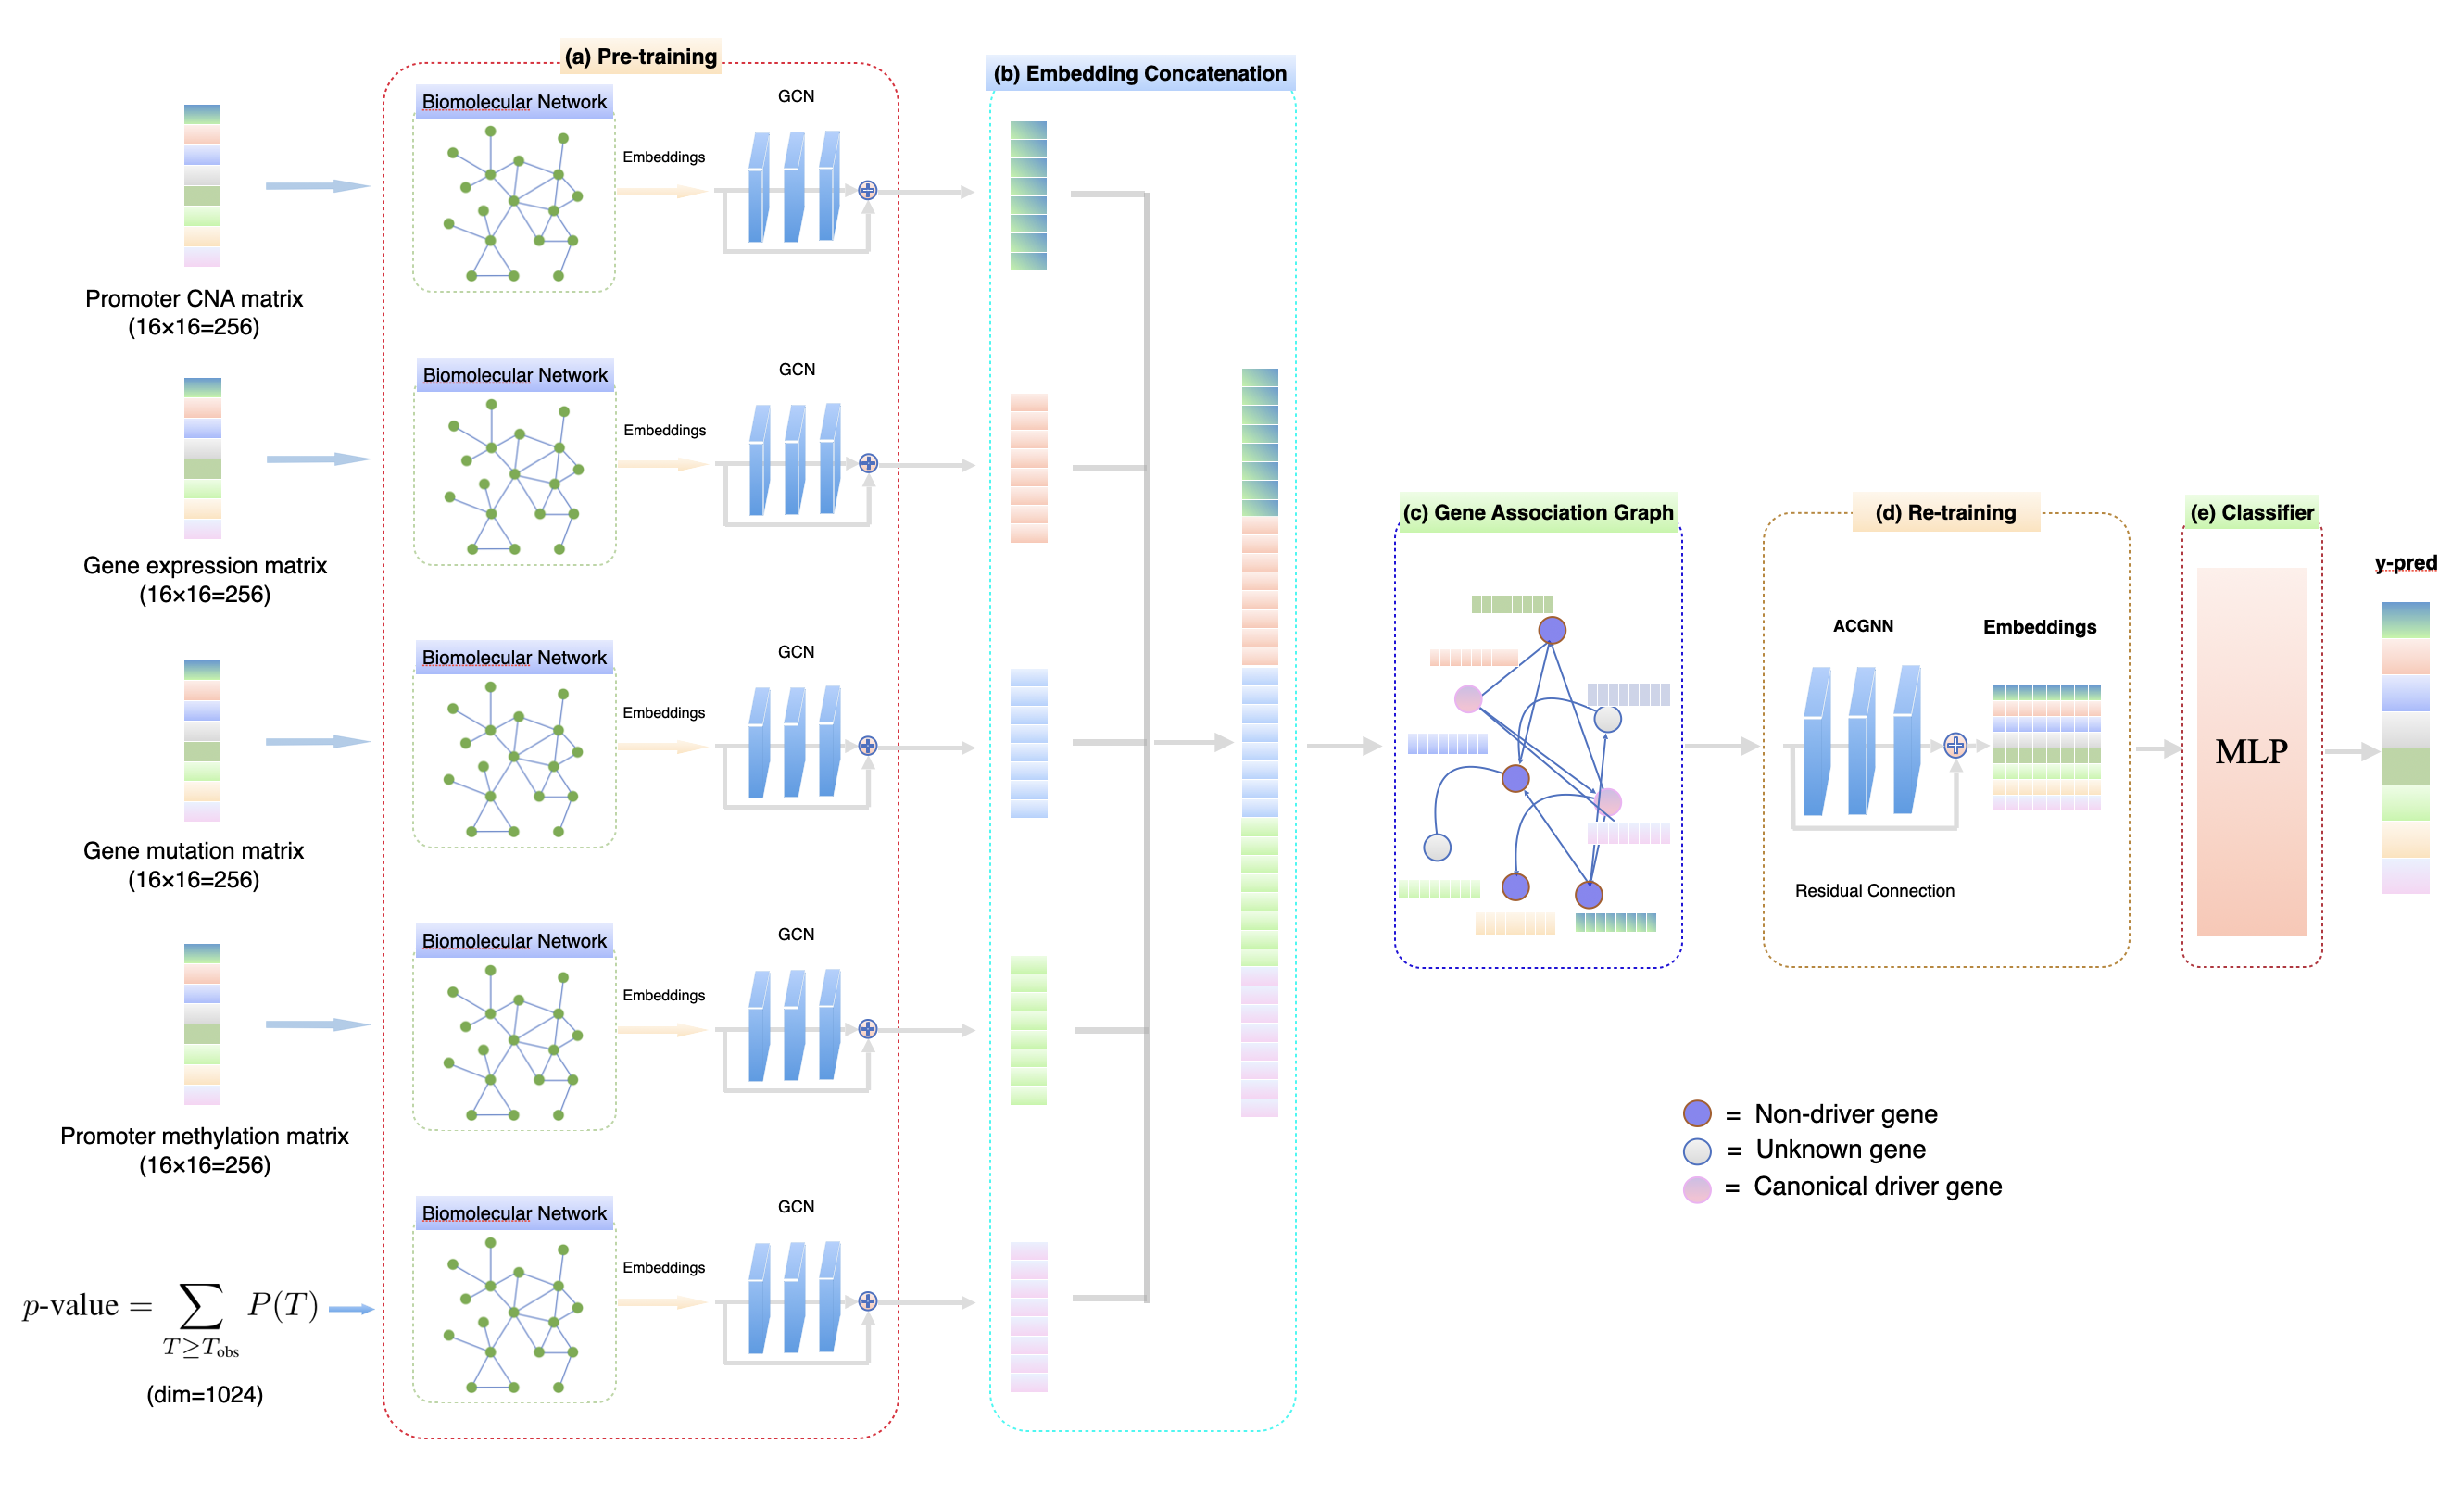
\includegraphics[width=18cm]{images/__overview_framework.png}
	%%\includegraphics[width=9.5cm]{images/_test_f1_vs_latent_dim_hid16_head4_lay8_epo1_5i298.png}
	\vspace{0.5cm} % Adjust the space as needed   
	\caption{Overview of the ACGNN framework.
		(a) Multi-omics biomolecular networks are constructed for gene expression, mutation, and promoter DNA methylation data. Embeddings are extracted using GCN, and PPI network embeddings are integrated through Fisher's exact test.
		(b) Multi-omics embeddings are concatenated to form unified feature representations, combining topological, statistical, and multi-omics data.
		(c) A gene embedding graph is created, where nodes represent genes, and edges capture relationships between concatenated embeddings.
		(d) The ACGNN model refines node embeddings using an adaptive mechanism that dynamically tunes the polynomial order and residual connections, producing low-dimensional representations.
		(e) A binary classifier predicts driver and non-driver genes, outputting probabilities for each gene.}
	\label{overview}
\end{figure*}

\subsection{Data Collection and Preprocessing}

In this study, we utilized the same PPI networks and multi-omics data as EMOGI and HGDC to evaluate our method's performance in identifying cancer driver genes. For completeness, we provide a brief overview of these datasets. 
The CPDB \cite{kamburov2011consensuspathdb} is a specialized database that integrates protein-protein interaction (PPI) data with cancer-specific annotations \cite{cpdb_citation}. It sources data from multiple experimental studies, such as The Cancer Genome Atlas (TCGA) \cite{tcga_citation}.
STRING combines data from high-throughput experiments and curated interaction databases \cite{string_citation}. This resource includes experimental data from sources like the Human Protein Atlas \cite{human_protein_atlas_citation}, KEGG \cite{kegg_citation}, Reactome pathways \cite{reactome_citation,wu2010human}, and Gene Ontology \cite{go_citation}.
HIPPIE (Human Integrated Protein-Protein Interaction Environment) focuses on human-specific protein interactions \cite{hippie_citation,alanis2017hippie,huang2018systematic,khurana2013interpretation}. It integrates high-quality experimental data and curated resources like the Molecular Interaction Database (MInt) \cite{mint_citation} and BioGRID \cite{biogrid_citation}.

The PPI Network, obtained from the STRING database \cite{szklarczyk2023string}, limited to high-confidence interactions with scores above 0.85. 
The multi-omics data, sourced from the TCGA database, included gene mutations, DNA methylation, and gene expression profiles. Similar to EMOGI and MNGCL, we focused on cancer types with available data for gene mutations, gene expression, and DNA methylation in both tumor and normal tissues. 

The three computed biological feature indices for genes are the gene mutation rate, the differential DNA methylation rate, and the differential gene expression rate. The gene mutation rate is calculated as the average of single nucleotide variations and copy number aberrations across all samples within a specific cancer type. The differential DNA methylation rate for each gene is calculated by averaging the methylation differences between cancer and normal samples. This averaging is performed across all cases for a given cancer type.
For each gene \(i\) in cancer type \(c\), a measure of dfferential DNA methylation (\(dm_{ci}\)) at its promoter can be defined as the difference in methylation signal between tumor (\(\beta_{ti}\)) and matched normal sample (\(\beta_{ni}\)), averaged across all available samples \(S_c\) for that \(c\):  

\begin{equation}
	dm_{ci} = \frac{1}{|S_c|} \sum_{t \in S_c} (\beta_{ti} - \beta_{ni}),
	\label{eq:dm_ci}
\end{equation}

The differential expression rate of each gene for a specific cancer type is calculated as the log\(_2\) fold change between expression in cancer and matched normal samples, averaged across all samples. The gene expression data, sourced from Wang et al.~\cite{wang2018unifying} was quantile-normalized and batch-corrected using the ComBat method~\cite{johnson2007adjusting}. 


\subsection{Gene Enrichment Analysis}

Gene enrichment analysis was conducted to identify significant associations among genes using Fisher's Exact Test \cite{fisher1992}. The dataset, containing gene interactions, was analyzed to compute p-values for shared interaction partners between gene pairs. False discovery rates (FDR) were controlled using the Benjamini-Hochberg method \cite{benjamini1995controlling}, with adjusted p-values below 0.05 considered significant. Results included gene pairs, shared partners, p-values, and significance labels. 

\subsection{ACGNN}	
	The Adaptive Chebyshev Graph Neural Network (ACGNN) framework integrates four types of multi-omics data: gene expression, gene mutation, promoter DNA methylation, and copy number alterations (CNA). For each data type, a corresponding biomolecular network \( G_i = (V, E) \) is constructed, where \( V \) represents genes and \( E \) represents interactions. Node embeddings for each network are obtained using Chebyshev spectral filtering. The extracted embeddings capture essential molecular interactions within each data type (Figudetire~\ref{overview}(a)).
	
	To incorporate additional topological information, PPI network embeddings are computed using Fisher’s exact test on enrichment analysis based on gene sets, utilizing the p-value as a significance measure. These topological embeddings provide structural insights into gene interactions.
	
	For each type of multi-omics data, 16 cancer-specific datasets are used to compute node embeddings of size 16, leading to a 256-dimensional feature vector per data type:
	\begin{equation}
		\mathbf{H}_i = \text{Concat}(\mathbf{h}_1, \mathbf{h}_2, ..., \mathbf{h}_{16}) \in \mathbb{R}^{256}
	\end{equation}
	where \( \mathbf{h}_j \) represents the embedding from the \( j \)-th dataset. The four vectors from different omics sources are concatenated to form a 1024-dimensional feature representation:
	\begin{equation}
		\mathbf{H}_{\text{multi-omics}} = \text{Concat}(\mathbf{H}_{\text{GE}}, \mathbf{H}_{\text{GM}}, \mathbf{H}_{\text{DM}}, \mathbf{H}_{\text{CNA}}) \in \mathbb{R}^{1024}
	\end{equation}
	
	Finally, the integrated multi-omics representation is concatenated with the PPI network embeddings to incorporate additional structural information:
	\begin{equation}
		\mathbf{H}_{\text{final}} = \text{Concat}(\mathbf{H}_{\text{multi-omics}}, \mathbf{H}_{\text{topological}}) \in \mathbb{R}^{2048}
	\end{equation}
	This final 2048-dimensional embedding serves as the comprehensive node representation, integrating molecular and structural information into the graph model (Figure~\ref{overview}(b)).
	
	Using these embeddings, a gene embedding graph is constructed, where nodes represent genes and edges capture relationships between them (Figure~\ref{overview}(c)). The ChebNet model refines the node representations through residual connections, which preserve the original feature information while enabling deeper feature transformations (Figure~\ref{overview}(d)).
	
	Finally, a binary classifier, implemented as a multi-layer perceptron (MLP) with a sigmoid activation function, predicts driver and non-driver genes (Figure~\ref{overview}(e)). The output is a probability score for each gene, representing its likelihood of being a cancer driver.
	

\begin{algorithm}
	\caption{ACGNN Method}
	\label{alg:acgnn}
	\textbf{Input:} Graph \( G = (V, E) \), node features \( \mathbf{H}^{(0)} \), rescaled Laplacian matrix \( \tilde{L} \), Chebyshev order \( k \), learnable weight matrices \( \Theta_j \), model parameters.\\
	\textbf{Output:} Predicted output \( Y \).
	
	\begin{algorithmic}[1]
		\State \textbf{Initialize:} Node features \( \mathbf{H}^{(0)} \) and Laplacian matrix \( \tilde{L} \).
		\State \( T_0(\tilde{L}) \leftarrow I \), \( T_1(\tilde{L}) \leftarrow \tilde{L} \)
		
		\For{\( j = 2 \) to \( k \)} \Comment{Compute Chebyshev polynomials}
		\State \( T_j(\tilde{L}) \leftarrow 2\tilde{L} T_{j-1}(\tilde{L}) - T_{j-2}(\tilde{L}) \)
		\EndFor
		
		\State \(\mathbf{H}^{(l+1)} \leftarrow \text{ReLU}\left( \sum_{j=0}^{k} \Theta_j T_j(\tilde{L}) \mathbf{H}^{(l)} \right) \)
		
		\State \(\mathbf{H}^{(l+1)} \gets \text{BatchNorm}(\mathbf{H}^{(l+1)})\)
		\State \(\mathbf{H}^{res} \gets \mathbf{H}^{(l+1)}\)  \Comment{Store residual connection}
		\State \(\mathbf{H}^{(l+2)} \gets \text{ReLU}\left( \sum_{j=0}^{k} \Theta_j T_j(\tilde{L}) \mathbf{H}^{(l+1)} \right) \)
		\State \(\mathbf{H}^{(l+2)} \gets \mathbf{H}^{(l+2)} + \mathbf{H}^{res} \) \Comment{Add residual}
		\State \(\mathbf{H}^{(l+2)} \gets \text{Dropout}(\mathbf{H}^{(l+2)})\)
		\State \( Y \gets \text{MLP}(\mathbf{H}^{(l+2)}) \)
		
		\State \Return \( Y \)
	\end{algorithmic}
\end{algorithm}


\subsection{Model Training and Inference}
	We implement ACGNN using PyTorch and DGL. The network architecture consists of two Chebyshev convolution layers followed by a Multi-Layer Perceptron (MLP). First, bidirectional graphs are constructed for biomolecular networks, incorporating pretrained embeddings as node features. Node labels are assigned as follows: 1 for driver genes, 0 for non-driver genes, and -1 for unlabeled genes.
	
	To define the training and testing sets, we apply the following masking strategy: the training mask includes all labeled nodes, while the testing mask allows all nodes to be evaluated. To ensure computational stability, self-loops are added to the graph, enabling nodes with no incoming edges to maintain connectivity. The model's feature dimensions are configured as follows: the input feature dimension is set to 128, the hidden feature dimension to 128, and the output dimension to 1 for binary classification.

	We use focal loss function \cite{lin2018focal}, given by Equation~\ref{eq:focal_loss}, to extend the standard Binary Cross-Entropy (BCE) loss to address class imbalance by reducing the loss contribution from well-classified examples and focusing more on hard-to-classify samples.
\begin{equation}
	\begin{aligned}
		L_{\text{focal}} = & - \alpha \left( 1 - h \right)^\gamma y \log(h) \\
		& - (1 - \alpha) h^\gamma (1 - y) \log(1 - h).
	\end{aligned}
	\label{eq:focal_loss}
\end{equation}

where \( y \) is the ground truth label, \( h \) is the predicted probability after applying the sigmoid activation function, \( \alpha \) is a weighting factor that balances the positive and negative classes, and \( \gamma \) is a focusing parameter that adjusts the impact of easy versus hard examples. A higher value of \( \gamma \) reduces the relative loss contribution from well-classified samples, placing greater emphasis on misclassified ones. The term \( (1 - h)^\gamma \) scales down the loss for correctly classified positive samples, whereas \( h^\gamma \) does the same for negative samples.

	
	By incorporating these terms, focal loss mitigates the dominance of easily classified examples, ensuring that the model prioritizes learning from challenging cases. This is particularly useful in imbalanced datasets where the positive class, such as cancer driver genes, is significantly underrepresented compared to the negative class.
	
	Node features and graph data are passed through the model to compute logits, which are then used to calculate the training loss based on the ground truth labels for nodes identified by the training mask. Predictions are generated for all nodes by applying a sigmoid activation to the computed logits, yielding the probabilities of each node belonging to the positive class. The pseudocode for executing our model is provided in Algorithm~\ref{alg:acgnn}.
	

\setlength{\tabcolsep}{3pt}  % Reduce column spacing
\begin{table}[h!]
	\centering
	\captionsetup{font=small}
	\scriptsize
	\begin{tabular}{@{}l*{6}{>{\centering\arraybackslash}p{1.2cm}}@{}}
		\toprule
		\textbf{Method} & \textbf{Layers} & \textbf{Input} & \textbf{Hidden} & \textbf{Output} & \textbf{Params} \\ 
		\midrule
		ACGNN     & 5 & 2048 & 1024 & 1 & 7,346,177 \\ 
		HGDC      & 3 & 2048  & 1024 & 1 & 4,202,497 \\ 
		EMOGI     & 3 & 2048  & 1024 & 1 & 4,202,497 \\ 
		MTGCN     & 3 & 2048 & 1024 & 1 & 4,198,401 \\
		GCN       & 3 & 2048 & 1024 & 1 & 4,198,401  \\ 
		GAT       & 3 & 2048 & 1024 & 1 & 4,202,497  \\ 
		GraphSAGE & 3 & 2048 & 1024 & 1 & 7,344,129 \\
		GIN       & 3 & 2048  & 1024 & 1 & 6,297,601 \\ 
		Chebnet   & 3 & 2048 & 1024 & 1 & 10,489,857 \\ 
		\bottomrule
	\end{tabular}
	\caption{Details of model architectures across different methods.}
	\label{tab:model_arch}
\end{table}



\begin{table*}[ht]
	\centering
	\scriptsize
	%\captionsetup{font=scriptsize}
	\captionsetup{font=footnotesize}
	%\caption{Comparison of Models in CPU/GPU Usage and Time Cost per Epoch}
	\begin{tabular}{l*{6}{>{\centering\arraybackslash}p{1.8cm}}}
		\toprule
		\textbf{Model} & \multicolumn{2}{c}{\textbf{CPDB}} & \multicolumn{2}{c}{\textbf{STRING}} & \multicolumn{2}{c}{\textbf{HIPPIE}} \\
		\cmidrule(lr){2-3} \cmidrule(lr){4-5} \cmidrule(lr){6-7}
		& \textbf{CPU/GPU Usage} & \textbf{Time/Epoch} & \textbf{CPU/GPU Usage} & \textbf{Time/Epoch} & \textbf{CPU/GPU Usage} & \textbf{Time/Epoch} \\
		\midrule
		ACGNN    & 3.17M/87.51M & 0.0426s & 3.78M/87.04M & 0.0328s & 3.14M/87.51M & 0.0227s\\
		HGDC     & 3.28M/55.75M & 0.0573s & 3.13M/55.29M & 0.0227s & 3.73M/55.75M & 0.0358s \\
		EMOGI   & 3.23M/55.75M & 0.0573s & 3.08M/55.29M & 0.0348s & 3.61M/55.75M & 0.0227s \\
		MTGCN   & 3.22M/55.72M & 0.0497s & 3.12M/55.25M & 0.0301s & 3.25M/55.72M & 0.0490s \\
		GCN     & 3.23M/55.72M & 0.0470s & 3.11M/55.25M & 0.0329s & 3.33M/55.72M & 0.0429s\\
		GAT     & 3.23M/55.75M & 0.0880s & 3.11M/55.29M & 0.1417s & 3.27M/55.75M & 0.0626s\\
		GrpahSAGE     & 3.17M/87.49M & 0.0532s & 3.25M/87.02M & 0.0210s & 3.18M/87.49M & 0.0330s \\
		GIN     & 3.17M/87.50M  & 0.0528s & 3.26M/87.04M & 0.0213s& 3.20M/87.50M & 0.0378s \\
		ChebNet & 3.22M/119.32M & 0.0622s & 3.13M/118.79M & 0.0241s & 3.16M/119.32M & 0.0453s \\
		\bottomrule
	\end{tabular}
	\caption{Comparison of models in CPU/GPU usage and time cost per epoch on the different PPI networks: CPDB, STRING, and HIPPIE.}
	\label{tab:consume_gpu}
\end{table*}


\begin{table}[ht]
	\centering
	\scriptsize
%\captionsetup{font=scriptsize}
\captionsetup{font=footnotesize}
	\begin{tabular}{l*{6}{>{\centering\arraybackslash}p{0.8cm}}}
		\toprule
		\textbf{Method} & \multicolumn{2}{c}{\textbf{CPDB}} & \multicolumn{2}{c}{\textbf{STRING}} & \multicolumn{2}{c}{\textbf{HIPPIE}} \\
		\cmidrule(lr){2-3} \cmidrule(lr){4-5} \cmidrule(lr){6-7}
		& \textbf{AUROC} & \textbf{AUPRC} & \textbf{AUROC} & \textbf{AUPRC} & \textbf{AUROC} & \textbf{AUPRC} \\
		\midrule
		ACGNN & 0.9652 & 0.9783 & 0.9578 & 0.9738 & 0.9297 & 0.9597 \\
		HGDC & 0.6776 & 0.7288 & 0.7133 & 0.7740 & 0.6525 & 0.7634 \\
		EMOGI & 0.6735 & 0.7230 & 0.81846 & 0.8737 & 0.6672 & 0.7960 \\
		MTGCN & 0.6862 & 0.7712 & 0.7130 & 0.7878 & 0.6762 & 0.7785 \\
		GCN & 0.6915 & 0.7730 & 0.6688 & 0.7681 & 0.6708 & 0.7675 \\
		GAT & 0.6670 & 0.7086 & 0.8166 & 0.8791 & 0.6478 & 0.7496 \\
		GraphSAGE & 0.6664 & 0.7522 & 0.6166 & 0.7182 & 0.6571 & 0.7624 \\
		GIN & 0.5836 & 0.6405 & 0.5173& 0.5918 & 0.5844 & 0.6791 \\
		Chebnet & 0.8017 & 0.8622 & 0.8777 & 0.9159 & 0.7409 & 0.8443 \\
		\bottomrule
	\end{tabular}
	\caption{Performance comparison of different methods across three biological networks: CPDB (pathway-based network), STRING (protein-protein interaction network), and HIPPIE (high-confidence protein interaction network).}
	\label{tab:roc_pr}
\end{table}

\begin{table}[ht]
	\centering
	\scriptsize
%\captionsetup{font=scriptsize}
\captionsetup{font=footnotesize}
	\begin{tabular}{l*{6}{>{\centering\arraybackslash}p{0.8cm}}}
		\toprule
		& \multicolumn{2}{c}{\textbf{CPDB}} & \multicolumn{2}{c}{\textbf{STRING}} & \multicolumn{2}{c}{\textbf{HIPPIE}} \\
		\cmidrule(lr){2-3} \cmidrule(lr){4-5} \cmidrule(lr){6-7}
		& \textbf{AUROC} & \textbf{AUPRC} & \textbf{AUROC} & \textbf{AUPRC} & \textbf{AUROC} & \textbf{AUPRC} \\
		\midrule
		ACGNN & 0.9652 & 0.9783 & 0.9578 & 0.9738 & 0.9297 & 0.9597 \\
		AC256x1 & 0.9315& 0.9527 & 0.9054 & 0.9464 & 0.8551 & 0.9129 \\
		AC256x2 & 0.9382& 0.9610 & 0.9413 & 0.9630 & 0.9112 & 0.9378 \\
		AC256x4 & 0.9495& 0.9657 & 0.9489 & 0.9634 & 0.8934 & 0.9388 \\
		AC1024x1 & 0.8481 & 0.9045 & 0.8653 & 0.9182 & 0.9288 & 0.9504 \\
		\bottomrule
	\end{tabular}
	\caption{The ablation experimental results of the different networks.}
	\label{tab:roc_pr_ablate}
\end{table}



%\begin{figure}[H]
%	\centering
%	\includegraphics[width=0.7\textwidth]{images/ggnet_kde.png}
%	\caption{Kernel Density Estimation (KDE) plot illustrating the distribution of interaction degrees for predicted driver genes and other genes. The x-axis represents the inteaction degree, and the y-axis represents the density.}
%	\label{fig:kde_plot}
%\end{figure}	
%\bigskip
%\vspace{0.5cm} 
	
	%======================================================
	\section{Experiments}
	\label{sec:experiment}
%	%======================================================
	

\subsection{Baseline Methods}

To evaluate the performance of ACGNN in identifying cancer driver genes, we compared it against eight other methods. These included three state-of-the-art GCN-based approaches: EMOGI, MTGCN, and HGDC, which leverage multi-omics data as gene features and incorporate PPI networks to learn gene representations for cancer driver gene prediction. Additionally, we assessed five widely-used GNN methods: GCN~\cite{kipf2017semi}, GIN~\cite{xu2018powerful}, ChebNet~\cite{defferrard2016convolutional}, GraphSAGE~\cite{hamilton2017inductive}, and GAT~\cite{velickovic2018graph}, which are traditional graph neural network models that aggregate features from neighboring nodes and themselves in different manners to learn new representations. All methods, including ACGNN, were tested on three distinct PPI networks, using the same network structure and gene feature matrix \( X \in \mathbb{R}^{N \times 2048} \) as inputs. Here, \( N \) denotes the number of genes, and the pretrained embeddings are of dimension 2048, comprising four concatenated 256-dimensional bio-feature vectors (\( 256 + 256 + 256 + 256 \)) and a topological feature of dimension 1024. Details of the model architecture are provided in Table \ref{tab:model_arch}.

\subsection{Experiment Settings}

Our algorithm is implemented in Python 3.9, utilizing PyTorch 2.0.1 and PyTorch Geometric 2.3.1, within an environment that also includes DGL. The Adam optimizer is employed, and we use FocalLoss (\( \alpha = 0.25, \gamma = 2 \)) as the loss function. The learning rate is set to 0.001, with the number of training epochs fixed at 200 throughout all experiments, unless stated otherwise. All experiments were conducted on an Ubuntu server featuring an Intel CPU (2.4GHz, 128GB RAM) and an Nvidia RTX 4080 GPU. The time consumption and CPU/GPU usage for different methods are detailed in Table \ref{tab:consume_gpu}.


\subsection{Gene Embeddings Clustering}

The initial task performed using the obtained embeddings involved clustering the nodes within the gene association graph. The process began with dataset preparation and gene mapping, followed by configuring the model with specific parameters, such as the number of layers and embedding dimensions. During training, multiple epochs were executed, where each batch was processed by computing logits, calculating the loss using a binary cross-entropy function with class imbalance weighting, and updating model parameters through backpropagation using the Adam optimizer. After each epoch, validation was performed to evaluate model performance, and the best model was selected based on the validation loss.
Using the optimal model, the final node embeddings were generated, and cluster labels were assigned accordingly. These embeddings were further analyzed to extract cluster-specific insights, including the identification of significant nodes within each cluster. The final model state was saved to enable future use, providing a structured representation of the gene network through clustered node embeddings.
Figure~\ref{fig:heatmap_clustering} presents the hierarchical clustering of genes based on pretrained node embeddings of dimension 300. The heatmap visualizes gene expression patterns, with red and blue indicating high and low expression levels, respectively. 
The hierarchical clustering dendrograms at the top and left of the heatmap reveal distinct gene clusters, highlighting structural similarities among genes. The presence of highly correlated gene groups suggests that the embedding model effectively captures biologically meaningful relationships.
Notably, genes such as \textit{NUP37}, \textit{CD2AP}, and \textit{AKT1} form distinct subclusters, implying potential functional similarity or co-regulation. In contrast, genes like \textit{EGFR}, \textit{ATR}, and \textit{STAT3} are grouped in separate regions, potentially reflecting their involvement in distinct biological pathways.
The structure of the heatmap demonstrates that the pretrained embeddings provide an informative representation of gene features, facilitating downstream analyses such as functional enrichment and pathway analysis.


\begin{figure}
	\centering
	\scriptsize
	\captionsetup{font=scriptsize}
	%\captionsetup{font=footnotesize}
	%%\captionsetup{font=scriptsize}
	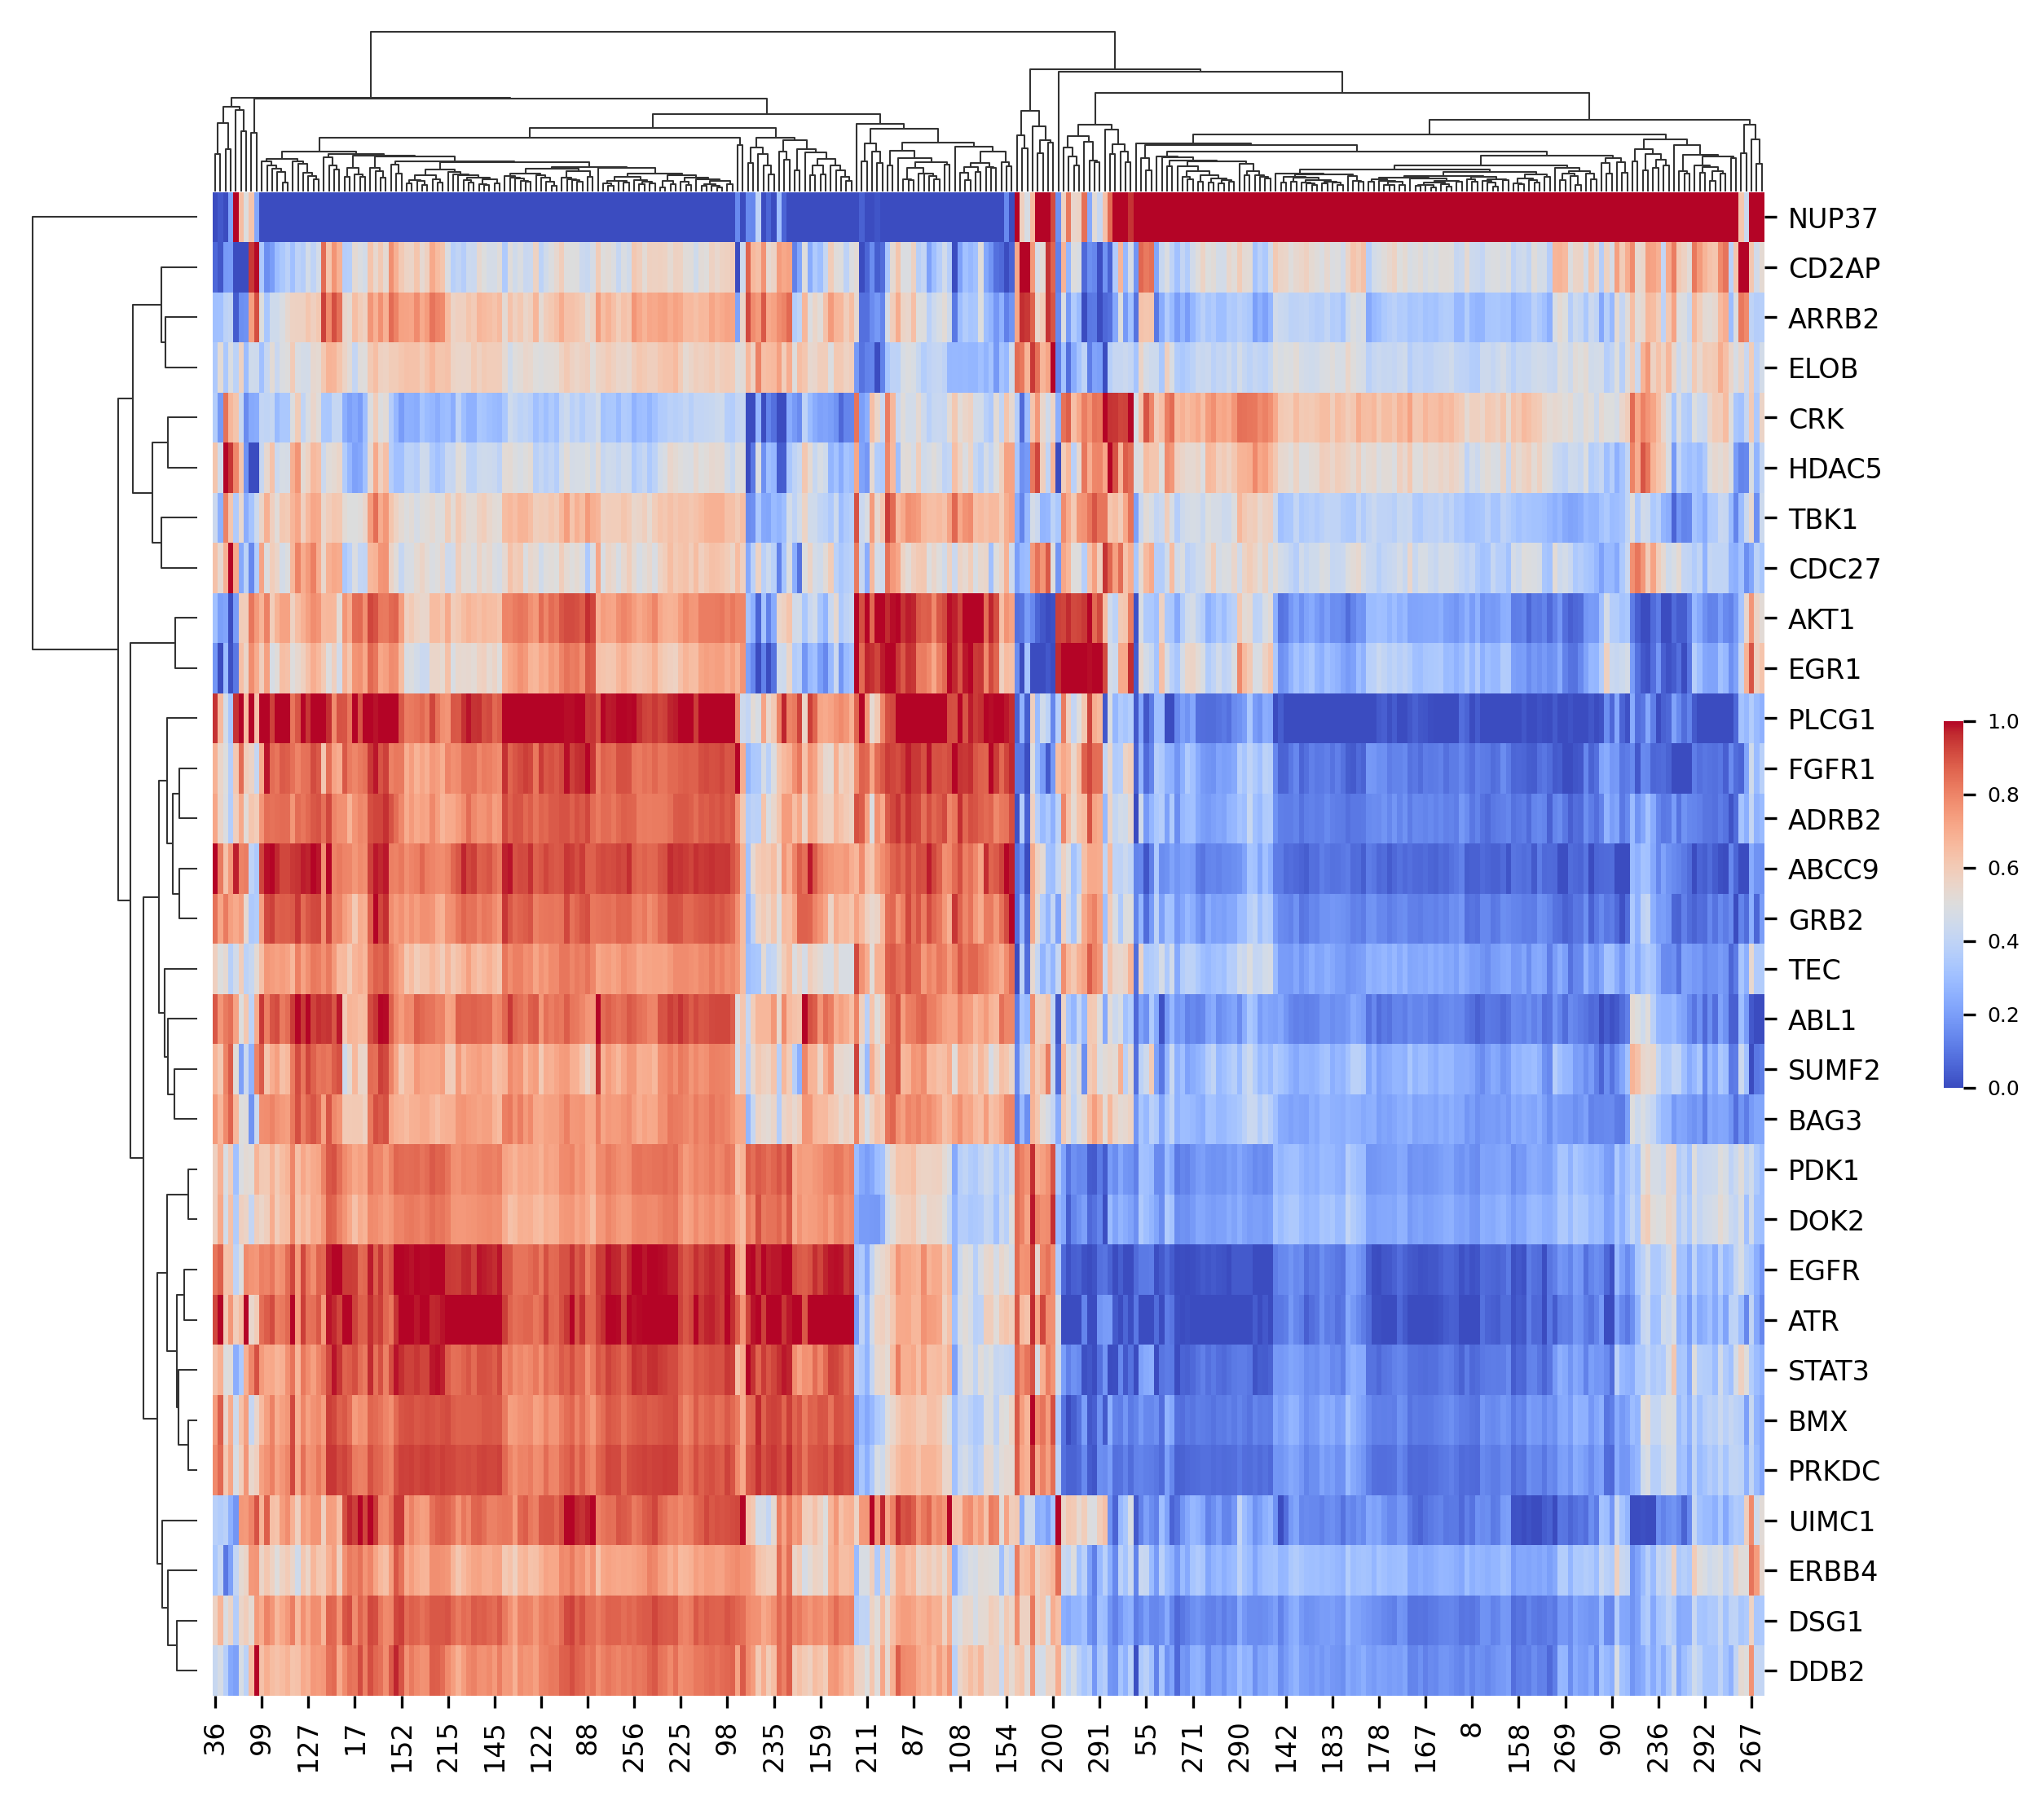
\includegraphics[width=0.49\textwidth]{images/KIRP_embeddings_matrix_stId_head2_dim16_lay2_epo100_.png}
	\caption{Demonstration of pretrained node embeddings with a dimension of 300 for clustering genes into k=30 clusters.}
	\label{fig:heatmap_clustering}
\end{figure}



%\vspace{0.5cm} % Adjust the space as needed 
\begin{figure}
	\centering
	%\captionsetup{font=scriptsize}
	\scriptsize
	%\captionsetup{font=scriptsize}
	\captionsetup{font=footnotesize}
	\subfloat[CPDB]{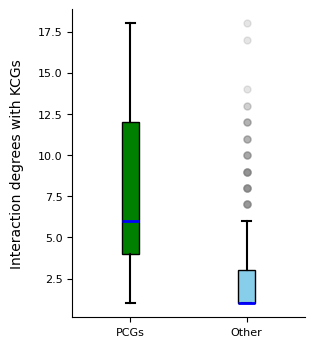
\includegraphics[width=1.2in]{images/__ACGNN_CPDB_degree_distributions_epo103_2048.png}}  
	\subfloat[STRING]{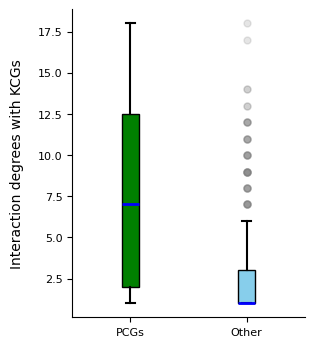
\includegraphics[width=1.2in]{images/__ACGNN_STRING_degree_distributions_epo103_2048.png}}
	\subfloat[HIPPIE]{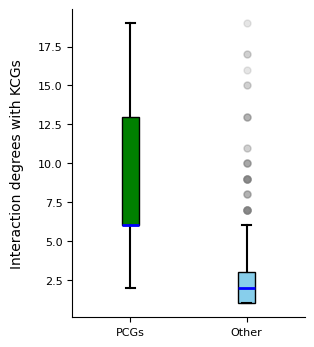
\includegraphics[width=1.2in]{images/__ACGNN_HIPPIE_degree_distributions_epo103_2048.png}}\\    
	\caption{The interaction distributions of Predicted Cancer Genes (PCGs) with Known Cancer Genes (KCGs) across three different protein-protein interaction (PPI) networks: CPDB, STRING, and HIPPIE.}
	\label{fig:degree}
\end{figure}

%\bigskip

\vspace{0.5cm} % Adjust the space as needed 
\begin{figure*}
	\centering
	%\captionsetup{font=scriptsize}
	\scriptsize
	%\captionsetup{font=scriptsize}
	\captionsetup{font=footnotesize}
	\subfloat[CPDB]{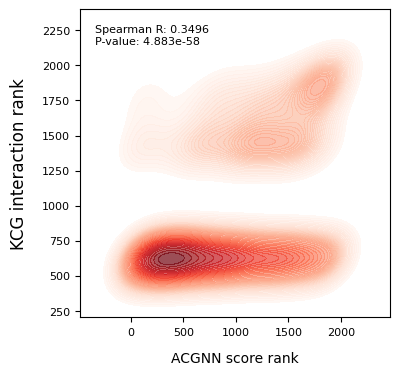
\includegraphics[width=2.0in]{images/CPDB_kde_plot_epo101_2048.png}}  
	\subfloat[STRING]{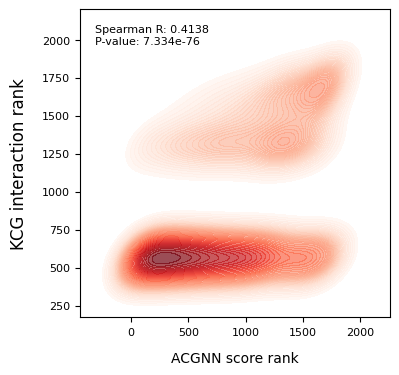
\includegraphics[width=2.0in]{images/STRING_kde_plot_epo101_2048.png}}
	\subfloat[HIPPIE]{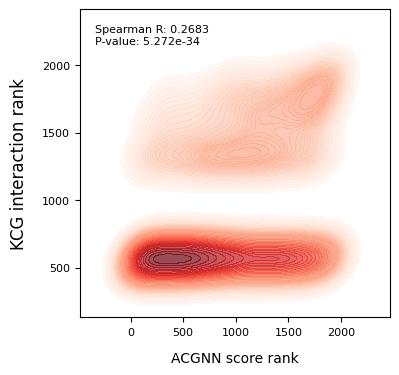
\includegraphics[width=2.0in]{images/HIPPIE_kde_plot_epo101_2048.png}}\\    
	\caption{Kernel Density Estimation (KDE) plot illustrating the distribution of interaction degrees for predicted driver genes and other genes. The x-axis represents the inteaction degree, and the y-axis represents the density.}
	\label{fig:kde_plot}
\end{figure*}


\begin{figure}[ht]
	\centering
	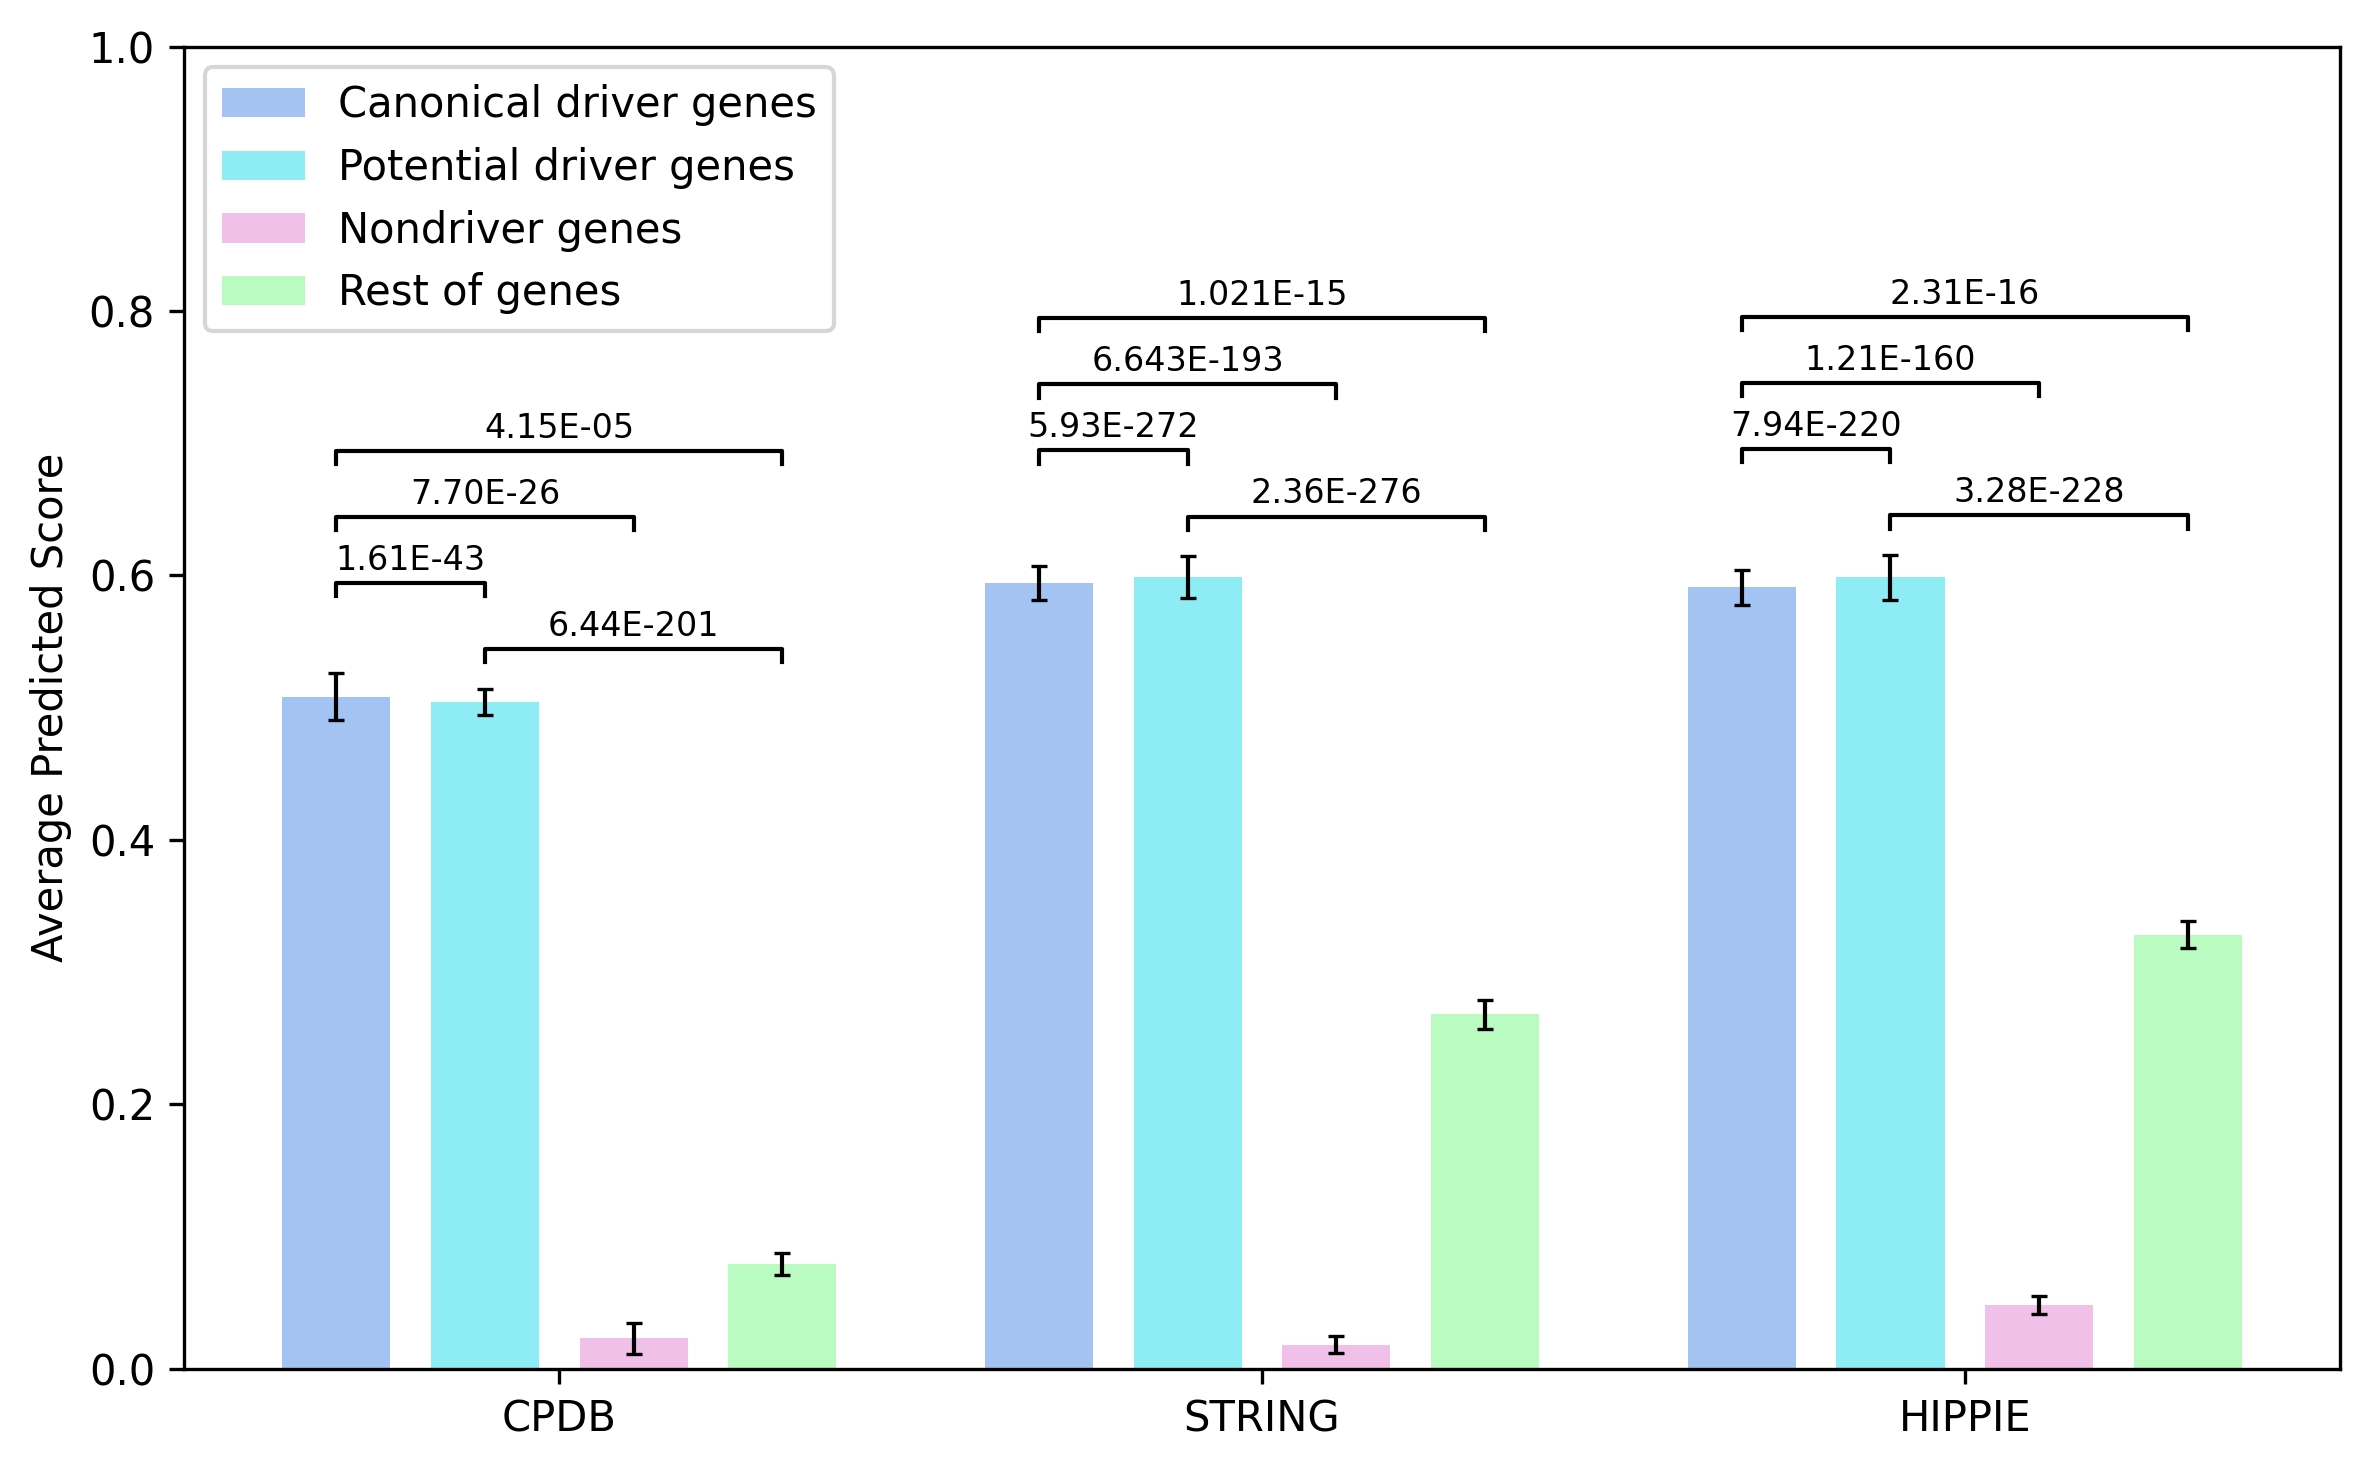
\includegraphics[width=0.45\textwidth]{images/average_predicted_scores.png}
	\captionsetup{font=footnotesize}
	\caption{Average predicted scores for different networks and gene types. The bar plot displays the scaled predicted scores for canonical driver genes, potential driver genes, nondriver genes, and the rest of the genes across three biological networks: CPDB, STRING, and HIPPIE. Error bars represent the scaled standard errors of the mean (SEM). The statistical significance (p-values) for comparisons between gene categories within each network is annotated above the bars. Numbers above the brackets represent the p-values of the Spearman Rank Correlation Test, indicating the significance of differences between groups.}
	
	\label{fig:predicted_scores}
\end{figure}


\begin{figure}[ht]
	\centering
		\scriptsize
	%\captionsetup{font=scriptsize}
	\captionsetup{font=footnotesize}
	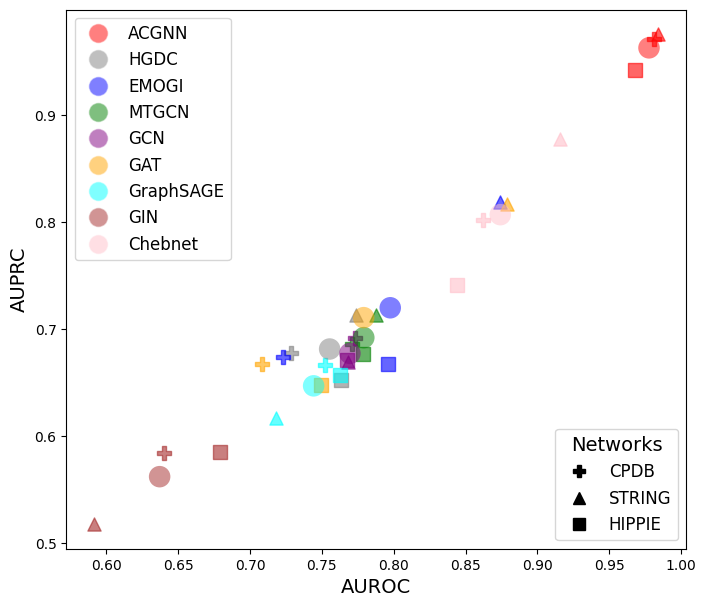
\includegraphics[width=0.45\textwidth]{images/roc_pr.png}
	\caption{
		Performance comparison of graph-based models across different biological networks. 
		The scatter plot shows the area under the receiver operating characteristic curve (AUROC) on the x-axis and the area under the precision-recall curve (AUPRC) on the y-axis for various models. The large circles represent the mean AUC values across biomolecular networks for each method.
	}
	\label{fig:auroc_auprc_comparison}
\end{figure}


\begin{figure}[ht]
	\centering
		\scriptsize
	%\captionsetup{font=scriptsize}
	\captionsetup{font=footnotesize}
	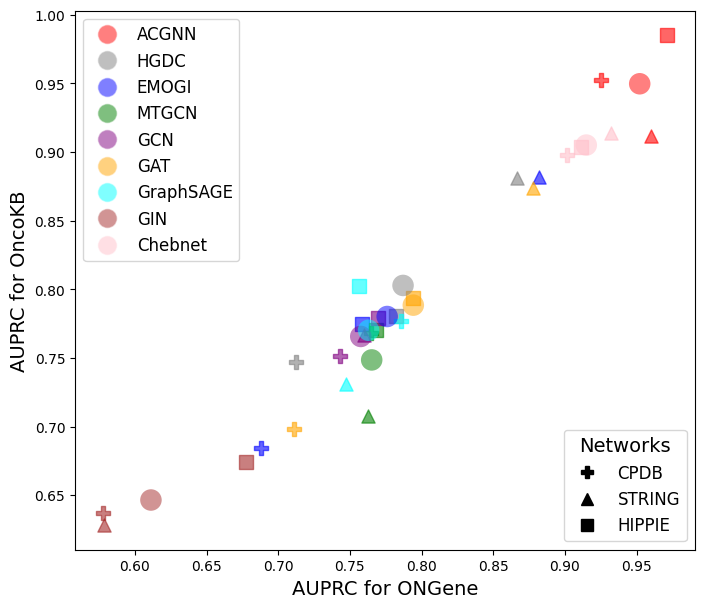
\includegraphics[width=0.45 \textwidth]{images/__comp_oncokb_ongene_acgnn.png}
	\caption{Performance comparisons of different methods on biomolecular networks. Results of all methods were evaluated on two independent test sets derived from the OncoKB and ONGene databases, respectively. The large circles represent the mean AUPRC values across biomolecular networks for each method.}
	\label{fig11}
\end{figure}



\subsection{Performance on Driver Gene Prediction}
We evaluated our method and baseline approaches for predicting driver genes on pan-cancer multi-omics dataset, using the average AUROC and AUPRC from ten iterations of validation as performance metrics. 
Figure~\ref{fig:auroc_auprc_comparison} presents the performance of various graph-based models on different biological networks. The x-axis represents the AUROC values, which indicate the classification ability of each model, while the y-axis represents the AUPRC values, highlighting precision-recall performance.
From the plot, ACGNN achieves the highest AUROC and AUPRC, indicating strong predictive performance. HGDC, EMOGI, and MTGCN exhibit competitive performance, clustering around an AUROC of 0.75–0.85. Different biomolecular networks (CPDB, STRING, HIPPIE) influence the model's performance, as seen from the varied shapes. GCN, GAT, and GraphSAGE show moderate results, suggesting dependency on network topology. 
The average results of ACGNN  and other eight methods on different biomolecular networks are also shown in Table~\ref{tab:roc_pr}. 

 Figure~\ref{fig11} compares the AUPRC performance of various methods across different biological networks using independent test sets from OncoKB and ONGene. The x-axis represents the AUPRC for ONGene, while the y-axis represents the AUPRC for OncoKB. 
ACGNN continues to outperform other models, achieving the highest scores across both test sets. HGDC, EMOGI, and MTGCN display competitive results, clustering between 0.75 and 0.85 AUPRC. The distribution of models across CPDB, STRING, and HIPPIE networks indicates variations in predictive performance due to differences in biological network structures.
The results demonstrate that methods leveraging advanced GNN architectures, particularly ACGNN, provide superior predictions in cancer driver gene identification compared to traditional models.


Figure~\ref{fig:degree} presents the interaction distributions of Predicted Cancer Genes (PCGs) with Known Cancer Genes (KCGs) across three different protein-protein interaction (PPI) networks: CPDB, STRING, and HIPPIE. The boxplots illustrate the interaction degrees between these gene categories, offering insights into their connectivity patterns.
In the CPDB network (Figure~\ref{fig:degree} a), PCGs exhibit a wider distribution of interaction degrees, with a higher median and several outliers. This suggests that PCGs in CPDB tend to have stronger connectivity with KCGs. The STRING network (Figure~\ref{fig:degree} b) follows a similar pattern, though with slightly lower median values and fewer extreme outliers, indicating a moderate connectivity between PCGs and KCGs. The HIPPIE network (Figure~\ref{fig:degree} c) displays the highest median interaction degree among the three networks, suggesting that it might capture a denser set of biologically relevant interactions for PCGs.
Across all three networks, PCGs demonstrate significantly higher interaction degrees with KCGs compared to other genes. The interquartile range (IQR) and median values for PCGs are consistently larger, while the presence of multiple outliers suggests that some PCGs have exceptionally high connectivity with KCGs. In contrast, the Other gene category has a much lower and more compact distribution, indicating weaker associations with KCGs.
These results reinforce the relevance of PCGs in cancer research, as their strong connectivity with known cancer genes suggests potential biological significance. The differences observed across the three networks highlight the impact of network-specific interaction curation, with HIPPIE capturing the densest set of interactions. 

Kernel Density Estimation (KDE) (Figure~\ref{fig:kde_plot}) presents the average predicted scores for different gene types across the three biological networks. The bar plot categorizes genes into canonical driver genes, potential driver genes, nondriver genes, and the rest of the genes. The error bars represent the scaled standard errors of the mean (SEM), ensuring statistical robustness in the displayed values.
Across all three networks, canonical driver genes consistently exhibit the highest predicted scores, followed by potential driver genes, while nondriver genes and the rest of the genes have significantly lower scores. This pattern suggests a strong alignment between the model’s predictions and known biological classifications of driver genes.
The statistical significance of the differences in predicted scores is annotated above the bars, with p-values from the Spearman Rank Correlation Test. The highly significant p-values (e.g., \( p < 10^{-40} \) in CPDB and similar magnitudes in STRING and HIPPIE) indicate strong differentiation between gene categories, reinforcing the predictive power of the model in distinguishing cancer-related genes.
Additionally, STRING and HIPPIE networks exhibit a greater separation between gene categories than CPDB, suggesting that these networks may capture more biologically relevant interactions. The increased predicted scores for the "rest of the genes" category in HIPPIE compared to CPDB and STRING could indicate a broader connectivity pattern in HIPPIE's network structure.
These results highlight the model’s ability to predict meaningful biological classifications across different interaction networks, with STRING and HIPPIE demonstrating particularly strong discriminatory power.


	

\subsection{Performance on OncoKB and ONGene}
To investigate whether the models’ performance is biased toward a specific dataset, we evaluated them on two additional cancer gene databases: OncoKB~\cite{chakravarty2017oncokb} and ONGene~\cite{liu2017ongene}. The cancer gene sets from OncoKB and ONGene are compiled from scientific literature or clinical studies and are therefore not explicitly informed by any of the data types used to train ACGNN . This demonstrates ACGNN 's capability to predict cancer genes broadly, independent of the methods or data used to define them, across the Gene Network, Pathway Network, and Protein-Protein Interaction Network. For this evaluation, the test set was masked exclusively for non-labeled genes.

The performance comparisons of different methods across biomolecular networks are illustrated in Figure~\ref{fig11}. A clear positive correlation between AUPRC values for the ONGene and OncoKB datasets is observed, indicating that methods performing well on one dataset tend to perform well on the other. This highlights the robustness and generalizability of certain methods across diverse, independent cancer gene sets.
Among the evaluated methods, ACGNN  achieves the highest performance on both datasets, as reflected by its red markers clustered near the top-right corner of the plot. Furthermore, ACGNN  maintains consistently high average AUPRC values, underscoring its reliability in network-based cancer gene prediction tasks.
These results emphasize the critical importance of integrating multiple biomolecular networks and leveraging advanced graph-based models for accurately identifying cancer driver genes. The alignment between the results from the OncoKB and ONGene datasets further validates the relevance and applicability of these methods in advancing cancer research.
 


\subsection{Feature Ablation Experiment}

The feature ablation experiments provide insights into the influence of different multi-omics data and biomolecular networks on the performance of ACGNN, as shown in Table \ref{tab:roc_pr_ablate}.
The table presents the ablation study results for different network variants trained on three biological networks: CPDB, STRING, and HIPPIE. The models tested include ACGNN, AC256x1, AC256x2, AC256x4, and AC1024x1. 
 ACGNN, the full model incorporating all bio-features and topological information, achieves the highest AUROC and AUPRC across all networks, demonstrating the advantage of integrating comprehensive features. AC256x1, using only one type of biological feature, and AC256x2, utilizing two types, show a decline in performance, indicating that limited biological features reduce predictive power. AC256x4, incorporating four types of biological features, performs better than AC256x2, suggesting that more bio-features enhance model performance. AC1024x1, which relies solely on topological information, has the lowest AUROC and AUPRC scores across most networks, confirming the critical role of biological features. These results highlight that incorporating multiple biological features significantly improves predictive accuracy, with the best performance achieved when combining all bio-features with topological information in ACGNN.

 
\subsection{Evaluation of Cancer Type-Specific Driver Gene Prediction}

We also investigate the effectiveness of ACGNN in detecting driver genes of a single cancer type. The results in Table \ref{tab:cancer_results} presents the AUROC (Area Under the Receiver Operating Characteristic Curve) and AUPRC (Area Under the Precision-Recall Curve) scores for various cancer types using four different methods: HGDC, EMOGI, MTGCN, and ACGNN. These metrics assess the predictive performance of each model across three feature types: biological (Bio), topological (Topo), and combined (Comb).
ACGNN consistently outperforms the other methods across all cancer types. The bolded values in the table indicate that ACGNN achieves the highest AUROC and AUPRC scores in nearly all cases, highlighting its effectiveness in predicting miRNA-disease associations compared to HGDC, EMOGI, and MTGCN. For instance, in bladder cancer (BLCA), ACGNN with combined features achieves an AUROC of 0.9644 and an AUPRC of 0.9766, significantly surpassing the next best method, MTGCN (Comb), which records an AUROC of 0.7525 and an AUPRC of 0.8174.

The integration of biological and topological features (Comb) consistently yields the best performance across all cancer types. In most cases, the AUROC and AUPRC values for the combined feature type are the highest, indicating that incorporating both biological and topological information enhances predictive accuracy. For example, in liver cancer (LIHC), ACGNN with combined features achieves an AUROC of 0.9704 and an AUPRC of 0.9809, outperforming the biological-only (AUROC = 0.9073, AUPRC = 0.9391) and topological-only (AUROC = 0.8513, AUPRC = 0.9022) configurations.
Certain methods exhibit limitations with specific cancer types. HGDC consistently performs the worst, frequently yielding the lowest AUROC and AUPRC values. While EMOGI and MTGCN produce competitive results in some cases, they are generally outperformed by ACGNN. For instance, in cervical cancer (CESC), HGDC with topological features achieves an AUROC of 0.6635 and an AUPRC of 0.7085, considerably lower than ACGNN with combined features, which attains an AUROC of 0.9760 and an AUPRC of 0.9871.
The superior performance of ACGNN across multiple cancer types suggests strong generalizability. 

 
  \subsection{Prediction of Novel Cancer Driver Genes}
  
To identify novel cancer driver genes, we trained the model using the CPDB network on the full training dataset with 500 epochs. Predictions were filtered by applying a threshold of 0.99, ensuring that only potential cancer driver genes were included while excluding previously labeled genes. This process resulted in 352 predicted cancer driver genes, of which 55 are already known cancer drivers. Additionally, 204 of the novel predictions have at least one supporting piece of evidence suggesting their potential as cancer drivers, based on sources such as NCG’s candidate cancer genes \cite{Repana2019}, OncoKB’s manually curated cancer genes, ONGene’s literature-curated cancer genes, and IntOGen's catalog of cancer-related mutations \cite{martinez2020compendium}. Among the top 60 predicted novel driver genes, 71.67\% (43 out of 60) have at least one supporting source indicating their potential role in cancer (Table \ref{table:gene_sources}).
 
 	\begin{table*}[h]
 	\centering
 	\begin{tabular}{llllll}
 		\toprule
 		\textbf{Gene} & \textbf{Confirmed Sources} & \textbf{Gene} & \textbf{Confirmed Sources} & \textbf{Gene} & \textbf{Confirmed Sources} \\
 		\midrule
 		ACTB & OncoKB, NCG, IntOGen & VDAC1 &  & SRP68 & IntOGen \\
 		CXCL2 & OnGene & BMP1 & IntOGen & CHMP6 &  \\
 		TRAF2 & OncoKB, NCG, IntOGen & CDK2 &  & DDB1 & IntOGen \\
 		RBBP4 & IntOGen & CRKL & OncoKB, OnGene & FHL2 & OnGene \\
 		UBC & IntOGen & KAT2B &  & HCK & IntOGen \\
 		LIN37 &  & ATR & OncoKB, NCG, IntOGen & ZWINT & NCG \\
 		FREM2 & NCG, IntOGen & CHRD & IntOGen & ACTN2 & IntOGen \\
 		LEF1 & OncoKB, OnGene, NCG, IntOGen & SIAE &  & DAXX & OncoKB, OnGene, NCG, IntOGen \\
 		PEX5 &  & UBXN7 & NCG & TEAD4 & IntOGen \\
 		ORC5 &  & TPM3 & OncoKB, NCG & RBM39 & NCG, IntOGen \\
 		NFKB1 & IntOGen & ABHD5 &  & HDAC1 & OncoKB, OnGene, NCG \\
 		HDAC2 & OncoKB, NCG & BIRC2 & OnGene & GRB2 & NCG, IntOGen \\
 		FOXK1 & NCG & GAB1 & OncoKB & EGFR & OncoKB, OnGene, NCG, IntOGen \\
 		PURA &  & TPM1 &  & KAT5 &  \\
 		HDAC3 & IntOGen & RBL1 & IntOGen & ATF5 & IntOGen \\
 		PRKDC & OncoKB, NCG, IntOGen & CDK9 &  & MYOM1 & IntOGen \\
 		NUP37 &  & TBP & NCG, IntOGen & ERCC6 & NCG, IntOGen \\
 		CDC20 & NCG & TBCA &  & GNA13 & OncoKB, OnGene, NCG, IntOGen \\
 		CASP7 &  & PLK1 & OnGene, NCG, IntOGen & SF3B3 & NCG \\
 		TRAF6 & OnGene, NCG, IntOGen & HDHD3 & IntOGen & UBE2B &  \\
 		\bottomrule
 	\end{tabular}
\caption{The top 60 predicted driver genes along with their confirmed sources, with unconfirmed genes left blank. Among these, 71.67\% of the novel genes have at least one supporting piece of evidence indicating their potential as cancer drivers. In total, 43 out of 60 genes are confirmed.}
 	\label{table:gene_sources}
 \end{table*}
 
 
	
	%======================================================
	\section{Discussion and Conclusions}
	\label{sec:conclusion}
	%======================================================
	Many genes exhibit context-dependent functions, being recurrently mutated in some cancers while undergoing epigenetic alterations in others \cite{baylin2016epigenetic,bell2019principles,repana2019ncg}.
To gain a comprehensive understanding of the cancer landscape, we emphasize the importance of integrating diverse molecular data types into a unified model for accurately predicting cancer genes with distinct characteristics.
ACGNN provides a scalable and adaptive framework for cancer gene prediction by leveraging Chebyshev polynomials, attention-based receptive fields, and pan-cancer multi-omics data integration. 
We evaluated the performance of ACGNN  across multiple cancer gene sets and PPI networks, comparing it with other established methods. While no single method consistently outperformed the others across all scenarios, ACGNN  trained on pan-cancer data demonstrated, on average, superior AUPRC values. 

While ACGNN  demonstrated stable performance across various cancer gene datasets, the performance of cancer driver gene prediction was highly dependent on the dataset used. This variability likely reflects the differing biases inherent in the collection of these cancer gene sets. For instance, the PPIs from STRING includes functional associations (e.g., co-expression or shared pathways) that do not necessarily indicate direct physical interactions between proteins. 

The ACGNN  framework is highly versatile, capable of integrating various types of omics data and networks beyond those utilized here. This flexibility allows its application beyond the field of cancer genomics, enabling the study of other complex diseases where multi-omics data are available, and functional gene connections play a critical role in classifying disease-related genes. Our future work will explore hybrid models combining ChebNet with Transformers.



\begin{table*}[h]
	\centering
	\renewcommand{\arraystretch}{1.1} % Slightly reduce row height
	\setlength{\tabcolsep}{3pt} % Reduce column spacing
	\small % Reduce font size
	\begin{tabular}{c l ccc ccc  c l ccc ccc}
		\toprule
		\multirow{2}{*}{\textbf{Cancer}} & \multirow{2}{*}{\textbf{Method}} & 
		\multicolumn{3}{c}{\textbf{AUROC}} & \multicolumn{3}{c}{\textbf{AUPRC}} &
		\multirow{2}{*}{\textbf{Cancer}} & \multirow{2}{*}{\textbf{Method}} & 
		\multicolumn{3}{c}{\textbf{AUROC}} & \multicolumn{3}{c}{\textbf{AUPRC}} \\
		\cmidrule(lr){3-5} \cmidrule(lr){6-8} \cmidrule(lr){11-13} \cmidrule(lr){14-16}
		& & \textbf{Bio} & \textbf{Topo} & \textbf{Comb} & \textbf{Bio} & \textbf{Topo} & \textbf{Comb} & 
		& & \textbf{Bio} & \textbf{Topo} & \textbf{Comb} & \textbf{Bio} & \textbf{Topo} & \textbf{Comb} \\
		\midrule
		% Left Group
		\multirow{4}{*}{BLCA} & HGDC & 0.7371 & 0.7130 & 0.7240 & 0.7957 & 0.7382 & 0.7837  & 
		\multirow{4}{*}{LIHC} & HGDC & 0.6939 & 0.6463 & 0.6724 & 0.7632 & 0.7037 & 0.7465 \\
		& EMOGI & 0.6335 & 0.7404 & 0.7698 & 0.6812 & 0.7903 & 0.8011  & 
		& EMOGI & 0.7215 & 0.7263 & 0.7136 & 0.7595 & 0.7866 & 0.7929 \\
		& MTGCN & 0.7491 & 0.6800 & 0.7525 & 0.8180 & 0.7677 & 0.8174 &  
		& MTGCN & 0.7235& 0.7022 & 0.8819 & 0.8110 & 0.7824 & 0.8523 \\
		& ACGNN & \textbf{0.8585} & \textbf{0.8507} & \textbf{0.9644} & \textbf{0.9079} & \textbf{0.9014} & \textbf{0.9766} & 
		& ACGNN & \textbf{0.9073} & \textbf{0.8513} & \textbf{0.9704} & \textbf{0.9391} & \textbf{0.9022} & \textbf{0.9809} \\
		\midrule
		% Add remaining cancers similarly in both columns
		\multirow{4}{*}{BRCA} & HGDC & 0.6406 & 0.5941 & 0.6980 & 0.7023& 0.6205 & 0.7249  & 
		\multirow{4}{*}{LUAD} & HGDC & 0.7260 & 0.6777 & 0.7149 & 0.7692 & 0.7297 & 0.7620 \\
		& EMOGI & 0.7539 & 0.7181 & 0.7127 & 0.8252 & 0.7816 & 0.7592  & 
		& EMOGI & 0.7351 & 0.7230& 0.7512 & 0.7825 & 0.7685 & 0.8196 \\
		& MTGCN & 0.7095 & 0.7145& 0.6853 & 0.7876 & 0.7906& 0.7705 & 
		& MTGCN & 0.6916 & 0.6918 & 0.7127 & 0.7828& 0.7724 & 0.7967 \\
		& ACGNN & \textbf{0.9017} & \textbf{0.8105} & \textbf{0.9287} & \textbf{0.9359} & \textbf{0.8714} & \textbf{0.9533} & 
		& ACGNN & \textbf{0.9384} & \textbf{0.8068} & \textbf{0.9026} & \textbf{0.9590} & \textbf{0.8704} & \textbf{0.9337} \\
		
		\midrule
		% Left Group
		\multirow{4}{*}{CESC} & HGDC & 0.6031 & 0.6635 & 0.7071 & 0.6765 & 0.7085 & 0.7663  & 
		\multirow{4}{*}{LUSC} & HGDC & 0.7030 & 0.6497 & 0.6589 & 0.7372 & 0.7119 & 0.6921 \\
		& EMOGI & 0.7592 & 0.7393 & 0.7196 & 0.8226 & 0.7823 & 0.7792 & 
		& EMOGI & 0.7761 & 0.6713 & 0.6724 & 0.8320 & 0.7278 & 0.7203 \\
		& MTGCN & 0.7272& 0.6969 & 0.7182 & 0.8060 & 0.7801 & 0.7984  & 
		& MTGCN & 0.7337& 0.6976 & 0.7010 & 0.8048 & 0.7824 & 0.7826 \\
		& ACGNN  & \textbf{0.9636}  & \textbf{0.7343}  & \textbf{0.9760}  & \textbf{0.9749}  & \textbf{0.8214}  & \textbf{0.9871}  & 
		& ACGNN  & \textbf{0.9569}  & \textbf{0.7995}  & \textbf{0.9282}  & \textbf{0.9716}  & \textbf{0.8666}  & \textbf{0.9510}  \\
		\midrule
		% Add remaining cancers similarly in both columns
		\multirow{4}{*}{COAD} & HGDC & 0.7364 & 0.6693 & 0.6849 & 0.7989 & 0.7205 & 0.7249 & 
		\multirow{4}{*}{PRAD} & HGDC & 0.7499 & 0.6984 & 0.7512 & 0.7840 & 0.7452 & 0.8134 \\
		& EMOGI & 0.6961 & 0.7492 & 0.7229 & 0.7260 & 0.7820 & 0.7751  & 
		& EMOGI & 0.7227 & 0.6942& 0.7495 & 0.7760 & 0.7404 & 0.7903 \\
		& MTGCN & 0.7458 & 0.7073 & 0.7400 & 0.8167 & 0.7886 & 0.8088  & 
		& MTGCN & 0.7441 & 0.6984 & 0.7023& 0.8140 & 0.7786 & 0.7858 \\
		& ACGNN  & \textbf{0.8672}  & \textbf{0.8467}  & \textbf{0.9376}  & \textbf{0.9034}  & \textbf{0.8990}  & \textbf{0.9565} & 
		& ACGNN  & \textbf{0.9108}  & \textbf{0.8073}  & \textbf{0.9466}  & \textbf{0.9423}  & \textbf{0.8675}  & \textbf{0.9654}  \\
		
		\midrule
		% Left Group
		\multirow{4}{*}{ESCA} & HGDC & 0.6980 & 0.6656 & 0.7482 & 0.7359 & 0.6874 & 0.8006  & 
		\multirow{4}{*}{READ} & HGDC & 0.7362 & 0.6040 & 0.6933 & 0.7753 & 0.6441 & 0.7448 \\
		& EMOGI & 0.7600 & 0.7627 & 0.7745 & 0.7939 & 0.8219 & 0.8208  & 
		& EMOGI & 0.7984 & 0.7276 & 0.7755 & 0.8451 & 0.7775 & 0.8199 \\
		& MTGCN & 0.7303 & 0.7000 & 0.7266& 0.7966 & 0.7807 & 0.7935 & 
		& MTGCN & 0.7215 & 0.6814 & 0.6934 & 0.8013 & 0.7740& 0.7828 \\
		& ACGNN  & \textbf{0.9490}  & \textbf{0.8005}  & \textbf{0.9757}  & \textbf{0.9672}  & \textbf{0.8640}  & \textbf{0.9845}  & 
		& ACGNN  & \textbf{0.9439}  & \textbf{0.8173}  & \textbf{0.9773}  & \textbf{0.9607}  & \textbf{0.8692}  & \textbf{0.9846}  \\
		\midrule
		% Add remaining cancers similarly in both columns
		\multirow{4}{*}{HNSC} & HGDC & 0.7067 & 0.7301 & 0.7404 & 0.7307 & 0.8105 & 0.7872  & 
		\multirow{4}{*}{STAD} & HGDC & 0.6896 & 0.6036 & 0.8673 & 0.7381 & 0.6569 & 0.7058 \\
		& EMOGI & 0.7131 & 0.7662 & 0.7073 & 07699 & 0.8272 & 0.7384  & 
		& EMOGI & 0.7557 & 0.7144 & 0.7545 & 0.8453& 0.7577 & 0.7881 \\
		& MTGCN & 0.7197 & 0.7045 & 0.7322 & 0.7937& 0.7803 & 0.7981 & 
		& MTGCN & 0.7305 & 0.7182 & 0.7110 & 0.8080 & 0.7940 & 0.7908 \\
		& ACGNN  & \textbf{0.9468}  & \textbf{0.8300}  & \textbf{0.9209}  & \textbf{0.9643}  & \textbf{0.8866}  & \textbf{0.9502}  & 
		& ACGNN  & \textbf{0.9439}  & \textbf{0.8042}  & \textbf{0.9560}  & \textbf{0.9628}  & \textbf{0.8719}  & \textbf{0.9721}  \\
		
		\midrule
		% Left Group
		\multirow{4}{*}{KIRC} & HGDC & 0.6861 & 0.6279 & 0.7195 & 0.7458 & 0.67973 & 0.7802  & 
		\multirow{4}{*}{THCA} & HGDC & 0.7152 & 0.6249 & 0.6734 & 0.7731 & 0.6916 & 0.7038 \\
		& EMOGI & 0.7285 & 0.6366 & 0.7480 & 0.7768 & 0.6995 & 0.7662 & 
		& EMOGI & 0.7226 & 0.7165 & 0.7519 & 0.7690 & 0.7739 & 0.8019 \\
		& MTGCN & 0.7260 & 0.7167 & 0.7159 & 0.8048 & 0.7924 & 0.7906  & 
		& MTGCN & 0.6751 & 0.7038 & 0.7410 & 0.7667 & 7865& 0.8083 \\
		& ACGNN  & \textbf{0.8862}  & \textbf{0.8643}  & \textbf{0.9617}  & \textbf{0.9212}  & \textbf{0.9073}  & \textbf{0.9739} & 
		& ACGNN  & \textbf{0.8550}  & \textbf{0.8312}  & \textbf{0.9088}  & \textbf{0.9011}  & \textbf{0.8832}  & \textbf{0.9416}  \\
		\midrule
		% Add remaining cancers similarly in both columns
		\multirow{4}{*}{KIRP} & HGDC & 0.6949 & 0.6895 & 0.6944 & 0.7416 & 0.7289 & 0.7477  & 
		\multirow{4}{*}{UCEC} & HGDC & 0.6596 & 0.6302 & 0.7559 & 0.7181 & 0.6734 & 0.8011 \\
		& EMOGI & 0.8170 & 0.6623 & 0.7000 & 0.8631 & 0.7056 & 0.7387  & 
		& EMOGI & 0.8164 & 0.7696 & 0.7917 & 0.8718 & 0.8144 & 0.8434 \\
		& MTGCN & 0.7023 & 0.7002 & 0.7227 & 0.7830 & 0.7829 & 0.7948  & 
		& MTGCN & 0.7371 & 0.7139 & 0.6608 & 0.8202 & 0.7924 & 0.7483 \\
		& ACGNN  & \textbf{0.8667}  & \textbf{0.7986}  & \textbf{0.9168}  & \textbf{0.9110}  & \textbf{0.8684}  & \textbf{0.9403}  & 
		& ACGNN & \textbf{0.9567} & \textbf{0.8029} & \textbf{0.9852} & \textbf{0.9718} & \textbf{0.8661} & \textbf{0.9902} \\
		
		% Continue filling remaining 6 types on each side similarly
		\bottomrule
	\end{tabular}
	\caption{Performance comparison on cancer type-specific driver gene prediction on CPDB network. 
		\textbf{Bio}: Biological features-based model. 
		\textbf{Topo}: Topological network features-based model. 
		\textbf{Comb}: Combined biological and topological features.}
	\label{tab:cancer_results}
\end{table*}


 
% \vspace{5cm} 

	
	\section*{Acknowledgements}
	\label{sec:acknowledgement}
	
%We sincerely thank the anonymous reviewers for their valuable suggestions and comments, which greatly improved this paper. Their feedback guided us in refining our approach and enhancing the clarity of the research. 
This work is supported by the National Science Foundation under Grant No. \text{2245805}.


\vspace{0.5cm} 

	
%%\clearpage
%%\clearpage
	%\section{References}
	\begin{thebibliography}{99}

%%Introduction

\bibitem{dees2012music}
N. D. Dees \textit{et al.}, ``MuSiC: Identifying Mutational Significance in Cancer Genomes,'' \textit{Genome Research}, vol. 22, pp. 1589–1598, 2012. doi: \url{10.1101/gr.134635.111}.

\bibitem{vogelstein2013cancer}
B. Vogelstein \textit{et al.}, ``Cancer Genome Landscapes,'' \textit{Science}, vol. 339, pp. 1546–1558, 2013. doi: \url{10.1126/science.1235122}.

\bibitem{leiserson2015pan}
M. D. M. Leiserson, F. Vandin, H.-T. Wu, \textit{et al.}, ``Pan-Cancer Network Analysis Identifies Combinations of Rare Somatic Mutations Across Pathways and Protein Complexes,'' \textit{Nature Genetics}, vol. 47, pp. 106–114, 2015. doi: \url{10.1038/ng.3168}.

\bibitem{weinstein2013tcga}
J. N. Weinstein \textit{et al.}, ``The cancer genome atlas pan-cancer analysis project,'' \textit{Nature Genetics}, vol. 45, no. 10, pp. 1113–1120, 2013.

\bibitem{bashashati2012drivernet}
A. Bashashati \textit{et al.}, ``DriverNet: Uncovering the impact of somatic driver mutations on transcriptional networks in cancer,'' \textit{Genome Biology}, vol. 13, no. 12, p. R124, 2012. doi: \url{10.1186/gb-2012-13-12-r124}.



\bibitem{lawrence2013mutational}
M. S. Lawrence \textit{et al.}, ``Mutational Heterogeneity in Cancer and the Search for New Cancer-Associated Genes,'' \textit{Nature}, vol. 499, pp. 214–218, 2013. doi: \url{10.1038/nature12213}.

\bibitem{alexandrov2013signatures}
L. B. Alexandrov \textit{et al.}, ``Signatures of Mutational Processes in Human Cancer,'' \textit{Nature}, vol. 500, pp. 415–421, 2013. doi: \url{10.1038/nature12477}.

\bibitem{hou2014dawnrank}
J. P. Hou and J. Ma, ``DawnRank: Discovering Personalized Driver Genes in Cancer,'' \textit{Genome Medicine}, vol. 6, no. 7, p. 56, 2014. doi: \url{10.1186/s13073-014-0056-8}.

\bibitem{repana2019network}
D. Repana \textit{et al.}, ``The Network of Cancer Genes (NCG): A Comprehensive Catalogue of Known and Candidate Cancer Genes from Cancer Sequencing Screens,'' \textit{Genome Biology}, vol. 20, pp. 1–12, 2019. doi: \url{10.1186/s13059-019-1760-7}.

\bibitem{sondka2018cosmic}
Z. Sondka \textit{et al.}, ``The COSMIC Cancer Gene Census: Describing Genetic Dysfunction Across All Human Cancers,'' \textit{Nature Reviews Cancer}, vol. 18, pp. 696–705, 2018. doi: \url{10.1038/s41568-018-0060-1}.

\bibitem{tamborero2013oncodriveclust}
D. Tamborero, A. Gonzalez-Perez, and N. Lopez-Bigas, ``Onco- driveCLUST: Exploiting the positional clustering of somatic mutations to identify cancer genes,'' \textit{Bioinformatics}, vol. 29, no. 18, pp. 2238–2244, Sep. 2013.

\bibitem{gillman2023identifying}
R. Gillman, M. A. Field, U. Schmitz, R. Karamatic, and L. Hebbard, ``Identifying cancer driver genes in individual tumours,'' \textit{Computational and Structural Biotechnology Journal}, vol. 21, pp. 5028–5038, 2023.

\bibitem{song2019identifying}
J. Song, W. Peng, F. Wang, and J. Wang, ``Identifying driver genes involving gene dysregulated expression, tissue-specific expression and gene-gene network,'' \textit{BMC Med. Genomics}, vol. 12, no. S7, p. 168, Dec. 2019.

\bibitem{peng2021identifying}
W. Peng, S. Yi, W. Dai, and J. Wang, ``Identifying and ranking potential cancer drivers using representation learning on attributed network,'' \textit{Methods}, vol. 192, pp. 13–24, Aug. 2021.

\bibitem{peng2022improving}
W. Peng, Q. Tang, W. Dai, and T. Chen, ``Improving cancer driver gene identification using multi-task learning on graph convolutional network,'' \textit{Briefings Bioinf.}, vol. 23, no. 1, Jan. 2022, Art. no. bbab432.


\bibitem{song2020entropy}
J. Song, W. Peng, and F. Wang, ``An entropy-based method for identifying mutual exclusive driver genes in cancer,'' \textit{IEEE/ACM Trans. Comput. Biol. Bioinf.}, vol. 17, no. 3, pp. 758–768, May 2020.

\bibitem{zhang2022dgmp}
S. W. Zhang, J. Y. Xu, and T. Zhang, ``DGMP: Identifying cancer driver genes by jointing DGCN and MLP from multi-omics genomic data,'' \textit{Genomics Proteomics Bioinformatics}, vol. 20, no. 5, pp. 928–938, Oct. 2022, doi: 10.1016/j.gpb.2022.11.004. Epub Dec. 1, 2022. PMID: 36464123; PMCID: PMC10025764.

\bibitem{cheng2016advances}
F. Cheng, J. Zhao, and Z. Zhao, ``Advances in computational approaches for prioritizing driver mutations and significantly mutated genes in cancer genomes,'' \textit{Briefings Bioinf.}, vol. 17, no. 4, pp. 642–656, Jul. 2016.

\bibitem{collier2019lotus}
O. Collier, V. Stoven, and J.-P. Vert, ``LOTUS: a single- and multitask machine learning algorithm for the prediction of cancer driver genes,'' \textit{PLoS Computational Biology}, vol. 15, 2019, Article e1007381. doi: \url{10.1371/journal.pcbi.1007381}.

\bibitem{yi2021graphrepresentation}
H.-C. Yi, Z.-H. You, D.-S. Huang, \textit{et al.}, ``Graph representation learning in bioinformatics: trends, methods and applications,'' \textit{Briefings in Bioinformatics}, vol. 23, 2021, Article bbab340. doi: \url{10.1093/bib/bbab340}.

\bibitem{mourikis2019cancer}
T. P. Mourikis, L. Benedetti, E. Foxall, \textit{et al.}, ``Patient-specific cancer genes contribute to recurrently perturbed pathways and establish therapeutic vulnerabilities in esophageal adenocarcinoma,'' \textit{Nature Communications}, vol. 10, p. 3101, 2019. doi: \url{10.1038/s41467-019-11069-0}.

\bibitem{nulsen2021pancancer}
J. Nulsen, H. Misetic, C. Yau, \textit{et al.}, ``Pan-cancer detection of driver genes at the single-patient resolution,'' \textit{Genome Medicine}, vol. 13, p. 12, 2021. doi: \url{10.1186/s13073-021-00820-7}.

\bibitem{scarselli2009graph}
F. Scarselli, M. Gori, A. C. Tsoi, M. Hagenbuchner, and G. Monfardini, ``The Graph Neural Network Model,'' \textit{IEEE Transactions on Neural Networks}, vol. 20, no. 1, pp. 61-80, Jan. 2009. doi: 10.1109/TNN.2008.2005605.


\bibitem{liu2022conversational}
X. Liu and M. Yang, ``Research on conversational machine reading comprehension based on dynamic graph neural network,'' \textit{Journal of Integrated Technology}, vol. 11, no. 2, pp. 67–78, 2022.

\bibitem{peng2022drugresponse}
W. Peng, T. Chen, and W. Dai, ``Predicting drug response based on multi-omics fusion and graph convolution,'' \textit{IEEE Journal of Biomedical and Health Informatics}, vol. 26, no. 3, pp. 1384–1393, Mar. 2022.

\bibitem{peng2022cancerdrugresponse}
W. Peng, H. Liu, W. Dai, N. Yu, and J. Wang, ``Predicting cancer drug response using parallel heterogeneous graph convolutional networks with neighborhood interactions,'' \textit{Bioinformatics}, vol. 38, no. 19, pp. 4546–4553, Sep. 2022.

\bibitem{albu2022approach}
A.-I. Albu, ``An approach for predicting protein-protein interactions using supervised autoencoders,'' \textit{Procedia Computer Science}, vol. 207, pp. 2023–2032, 2022, doi: 10.1016/j.procs.2022.09.261.



%% related works

\bibitem{chatzianastasis2023emgnn}
M. Chatzianastasis, M. Vazirgiannis, and Z. Zhang, ``Explainable Multilayer Graph Neural Network for Cancer Gene Prediction,'' \textit{Bioinformatics}, Oct. 2023. doi: \url{10.1093/bioinformatics/btad643}. Available: \url{https://doi.org/10.1093/bioinformatics/btad643}.

\bibitem{li2024multimodalgnn}
B. Li and S. A. Nabavi, ``A Multimodal Graph Neural Network Framework for Cancer Molecular Subtype Classification,'' \textit{BMC Bioinformatics}, vol. 25, p. 27, 2024. Available: \url{https://doi.org/10.1186/s12859-023-05622-4}.

\bibitem{li2023cgmega}
H. Li, Z. Han, Y. Sun, F. Wang, P. Hu, C. Ren, X. Xu, H. Chen, Y. Yang, and X. Bo, ``CGMega: Explainable Graph Neural Network Framework with Attention Mechanisms for Cancer Gene Module Dissection,'' 2023. doi: \url{10.21203/rs.3.rs-3180743/v1}. Available: \url{https://doi.org/10.21203/rs.3.rs-3180743/v1}.


\bibitem{peng2022cancerdriver}
W. Peng, Q. Tang, W. Dai, and T. Chen, ``Improving Cancer Driver Gene Identification Using Multi-task Learning on Graph Convolutional Network,'' \textit{Briefings in Bioinformatics}, vol. 23, no. 1, Article bbab432, Jan. 2022. Available: \url{https://doi.org/10.1093/bib/bbab432}.

\bibitem{peng2024multinetwork}
W. Peng, Z. Zhou, W. Dai, N. Yu, and J. Wang, ``Multi-Network Graph Contrastive Learning for Cancer Driver Gene Identification,'' \textit{IEEE Transactions on Network Science and Engineering}, vol. 11, no. 4, pp. 3430-3440, Jul.-Aug. 2024. doi: \url{10.1109/TNSE.2024.3373652}.


\bibitem{schulte2021multiomics}
R. Schulte-Sasse, S. Budach, D. Hnisz, and et al., ``Integration of Multiomics Data with Graph Convolutional Networks to Identify New Cancer Genes and Their Associated Molecular Mechanisms,'' \textit{Nature Machine Intelligence}, vol. 3, pp. 513–526, 2021. Available: \url{https://doi.org/10.1038/s42256-021-00325-y}. 


\bibitem{zhang2023heterophilic}
T. Zhang, S.-W. Zhang, M.-Y. Xie, and Y. Li, ``A Novel Heterophilic Graph Diffusion Convolutional Network for Identifying Cancer Driver Genes,'' \textit{Briefings in Bioinformatics}, vol. 24, no. 3, May 2023, bbad137. Available: \url{https://doi.org/10.1093/bib/bbad137}.

\bibitem{ivan2011web}
I. G. Iván and V. Grolmusz, ``When the Web Meets the Cell: Using Personalized PageRank for Analyzing Protein Interaction Networks,'' \textit{Bioinformatics}, vol. 27, no. 3, pp. 405–407, 2011. doi: \url{10.1093/bioinformatics/btq671}.


\bibitem{zhao2022modig}
W. Zhao, X. Gu, S. Chen, J. Wu, and Z. Zhou, ``MODIG: Integrating Multi-Omics and Multi-Dimensional Gene Network for Cancer Driver Gene Identification Based on Graph Attention Network Model,'' \textit{Bioinformatics}, vol. 38, no. 21, pp. 4901-4907, Oct. 2022. doi: \url{10.1093/bioinformatics/btac622}.


\bibitem{du2018topology}
J. Du, S. Zhang, G. Wu, J. M. F. Moura, and S. Kar, ``Topology adaptive graph convolutional networks,'' \textit{arXiv preprint}, vol. 1710, no. 10370, 2018. [Online]. Available: \url{https://arxiv.org/abs/1710.10370}.

\bibitem{singh2024gtagcn}
S. Singh, A. Sharma, and V. K. Chauhan, ``GTAGCN: Generalized Topology Adaptive Graph Convolutional Networks,'' \textit{arXiv}, Mar. 2024. Available: \url{https://arxiv.org/abs/2403.15077}.





%%% Materials

\bibitem{kamburov2011consensuspathdb}
Kamburov, A., Pentchev, K., Galicka, H., Wierling, C., Lehrach, H., \& Herwig, R. "ConsensusPathDB: toward a more complete picture of cell biology." \textit{Nucleic Acids Research}, vol. 39, Database issue, pp. D712-D717, 2011. \url{https://doi.org/10.1093/nar/gkq1156}.

\bibitem{cpdb_citation}
Li, Z., et al. "CPDB: A comprehensive cancer protein database." \textit{Bioinformatics}, vol. 33, no. 7, pp. 1073-1080, 2017.

\bibitem{tcga_citation}
Weinstein, J. N., et al. "The Cancer Genome Atlas Pan-Cancer analysis project." \textit{Nature Genetics}, vol. 45, no. 10, pp. 1113-1120, 2013.

\bibitem{string_citation}
Szklarczyk, D., et al. "STRING v11: protein-protein association networks with increased coverage, supporting functional discovery in genome-wide experimental datasets." \textit{Nucleic Acids Research}, vol. 47, no. D1, pp. D607-D613, 2019.

\bibitem{human_protein_atlas_citation}
Uhlén, M., et al. "The Human Protein Atlas: an integrated exploration of the human proteome." \textit{Cell}, vol. 162, no. 2, pp. 383-393, 2015.

\bibitem{kegg_citation}
Kanehisa, M., et al. "KEGG: Kyoto Encyclopedia of Genes and Genomes." \textit{Nucleic Acids Research}, vol. 28, no. 1, pp. 27-30, 2000.

\bibitem{reactome_citation}
Jassal, B., et al. "Reactome: a database of reactions, pathways and biological processes." \textit{Nucleic Acids Research}, vol. 48, no. D1, pp. D497-D503, 2020.


\bibitem{wu2010human}
G. Wu, X. Feng, and L. Stein, ``A human functional protein interaction network and its application to cancer data analysis,'' \textit{Genome Biology}, vol. 11, no. 5, p. R53, May 2010. doi: \url{10.1186/gb-2010-11-5-r53}. PMID: 20482850; PMCID: PMC2898064.

\bibitem{go_citation}
The Gene Ontology Consortium. "Gene Ontology: tool for the unification of biology." \textit{Nature Genetics}, vol. 25, no. 1, pp. 25-29, 2000.

\bibitem{hippie_citation}
Lopes, F. M., et al. "HIPPIE: a human integrated protein-protein interaction database." \textit{Nucleic Acids Research}, vol. 45, no. D1, pp. D207-D212, 2017.

\bibitem{alanis2017hippie}
Alanis-Lobato, G., Andrade-Navarro, M. A., and Schaefer, M. H. (2017). HIPPIE v2.0: enhancing meaningfulness and reliability of protein-protein interaction networks. \textit{Nucleic Acids Research}, 45(D1), D408–D414. https://doi.org/10.1093/nar/gkw985

\bibitem{huang2018systematic}
Huang, J. K., Carlin, D. E., Yu, M. K., Zhang, W., Kreisberg, J. F., Tamayo, P., and Ideker, T. "Systematic evaluation of molecular networks for discovery of disease genes." \textit{Cell Systems}, vol. 6, no. 4, pp. 484-495.e5, 2018. \url{https://doi.org/10.1016/j.cels.2018.03.001}.

\bibitem{khurana2013interpretation}
Khurana, E., Fu, Y., Chen, J., and Gerstein, M. (2013). Interpretation of genomic variants using a unified biological network approach. \textit{PLoS Computational Biology}, 9(3), e1002886. https://doi.org/10.1371/journal.pcbi.1002886

\bibitem{mint_citation}
Rual, J. F., et al. "MIntAct: an open source database and analysis environment for protein-protein interaction data." \textit{Nucleic Acids Research}, vol. 33, suppl. 1, pp. D225-D229, 2005.

\bibitem{biogrid_citation}
Chatr-Aryamontri, A., et al. "The BioGRID interaction database: 2015 update." \textit{Nucleic Acids Research}, vol. 43, no. D1, pp. D470-D478, 2015.

\bibitem{szklarczyk2023string}
D. Szklarczyk, R. Kirsch, M. Koutrouli, K. Nastou, F. Mehryary, R. Hachilif, A. L. Gable, T. Fang, N. T. Doncheva, S. Pyysalo, P. Bork, L. J. Jensen, and C. von Mering, ``The STRING database in 2023: protein-protein association networks and functional enrichment analyses for any sequenced genome of interest,'' \textit{Nucleic Acids Res}, vol. 51, no. D1, pp. D638-D646, Jan. 2023. doi: 10.1093/nar/gkac1000.


\bibitem{wang2018unifying}
Wang, Q., Armenia, J., Zhang, C., et al. "Unifying cancer and normal RNA sequencing data from different sources." \textit{Scientific Data}, vol. 5, 180061, 2018. \url{https://doi.org/10.1038/sdata.2018.61}.

\bibitem{johnson2007adjusting}
Johnson, W. E., Li, C., \& Rabinovic, A. "Adjusting batch effects in microarray expression data using empirical Bayes methods." \textit{Biostatistics}, vol. 8, no. 1, pp. 118–127, 2007. \url{https://doi.org/10.1093/biostatistics/kxj037}.


\bibitem{fisher1992}
R. A. Fisher, ``Statistical methods for research workers,'' in \textit{Breakthroughs in Statistics}, S. Kotz and N. L. Johnson, Eds., Springer Series in Statistics. New York, NY: Springer, 1992, pp. 66-70. doi: 10.1007/978-1-4612-4380-9.

\bibitem{benjamini1995controlling}
Y. Benjamini and Y. Hochberg, ``Controlling the False Discovery Rate: A Practical and Powerful Approach to Multiple Testing,'' \textit{Journal of the Royal Statistical Society, Series B: Statistical Methodology}, vol. 57, no. 1, pp. 289--300, 1995.


\bibitem{lin2018focal}
T.-Y. Lin, P. Goyal, R. Girshick, K. He, and P. Dollár, ``Focal Loss for Dense Object Detection,'' \textit{arXiv preprint}, 2018. Available: arXiv:1708.02002.

%% experiment


\bibitem{kipf2017semi}
Kipf, Thomas N., and Max Welling. "Semi-supervised classification with graph convolutional networks." arXiv preprint arXiv:1609.02907 (2017).


\bibitem{xu2018powerful}
K. Xu, W. Hu, J. Leskovec, and S. Jegelka, ``How Powerful are Graph Neural Networks?,'' \textit{ICLR}, 2019.

\bibitem{defferrard2016convolutional}
M. Defferrard, X. Bresson, and P. Vandergheynst, ``Convolutional Neural Networks on Graphs with Fast Localized Spectral Filtering,'' \textit{Advances in Neural Information Processing Systems}, vol. 29, pp. 3844--3852, 2016.

\bibitem{hamilton2017inductive}
Hamilton, William L., Rex Ying, and Jure Leskovec. "Inductive representation learning on large graphs." Advances in neural information processing systems 30 (2017).

\bibitem{velickovic2018graph}
P. Veličković, G. Cucurull, A. Casanova, A. Romero, P. Liò, and Y. Bengio, ``Graph Attention Networks,'' \textit{International Conference on Learning Representations}, 2018. Available: https://openreview.net/forum?id=rJXMpikCZ. [Accepted as poster].

%
%\bibitem{suehnholz2024clinical}
%S. P. Suehnholz \textit{et al.}, ``Quantifying the Expanding Landscape of Clinical Actionability for Patients with Cancer,'' \textit{Cancer Discovery}, vol. 14, no. 1, pp. 49–65, Jan. 2024. doi: \url{10.1158/2159-8290.CD-23-0467}. PMID: 37849038; PMCID: PMC10784742.

\bibitem{chakravarty2017oncokb}
D. Chakravarty \textit{et al.}, ``OncoKB: A Precision Oncology Knowledge Base,'' \textit{JCO Precision Oncology}, vol. 2017, p. PO.17.00011, Jul. 2017. doi: \url{10.1200/PO.17.00011}. PMID: 28890946; PMCID: PMC5586540.

\bibitem{liu2017ongene}
Y. Liu, J. Sun, and M. Zhao, ``ONGene: A literature-based database for human oncogenes,'' \textit{Journal of Genetics and Genomics}, vol. 44, no. 2, pp. 119–121, Feb. 2017. doi: \url{10.1016/j.jgg.2016.12.004}. PMID: 28162959.


\bibitem{ogata1999kegg}
Ogata H., Goto S., Sato K., Fujibuchi W., Bono H., Kanehisa M. "KEGG: Kyoto Encyclopedia of Genes and Genomes." \textit{Nucleic Acids Research}, vol. 27, no. 1, pp. 29–34, 1999. \url{https://doi.org/10.1093/nar/27.1.29}.


\bibitem{zhang2021edgeconv}
Zheng Zhang, Lei Cui, Jianping Wu. "Exploring an edge convolution and normalization based approach for link prediction in complex networks." \textit{Journal of Network and Computer Applications}, vol. 189, 103113, 2021. \url{https://doi.org/10.1016/j.jnca.2021.103113}.

\bibitem{zhang2024highfreq}
Zhang Z., Xu H., Zhu G. "Incorporating high-frequency information into edge convolution for link prediction in complex networks." \textit{Scientific Reports}, vol. 14, no. 1, p. 5437, 2024. \url{https://doi.org/10.1038/s41598-024-56144-9}.

\bibitem{Repana2019}
Repana, D. \textit{et al.} "The network of cancer genes (NCG): a comprehensive catalogue of known and candidate cancer genes from cancer sequencing screens." \textit{Genome Biology}, vol. 20, p. 1, 2019. \url{https://doi.org/10.1186/s13059-019-1701-7}.


\bibitem{martinez2020compendium}
Martínez-Jiménez, F., Muiños, F., Sentís, I., Deu-Pons, J., Reyes-Salazar, I., Arnedo-Pac, C., Mularoni, L., Pich, O., Bonet, J., Kranas, H., Gonzalez-Perez, A., \& Lopez-Bigas, N. "A compendium of mutational cancer driver genes." \textit{Nature Reviews Cancer}, vol. XX, pp. XXX–XXX, 2020. \url{https://doi.org/10.xxxx}.

%% discussion

\bibitem{bell2019principles}
Bell, C. C. \& Gilan, O. "Principles and mechanisms of non-genetic resistance in cancer." \textit{British Journal of Cancer}, vol. 122, pp. 465–472, 2019. \url{https://doi.org/10.1038}.
	
\bibitem{repana2019ncg}
Repana, D., et al. "The network of cancer genes (NCG): a comprehensive catalogue of known and candidate cancer genes from cancer sequencing screens." \textit{Genome Biology}, vol. 20, p. 1, 2019. \url{https://doi.org/10.1186/s13059-018-1612-0}.

\bibitem{baylin2016epigenetic}
Baylin, S. B. \& Jones, P. A. "Epigenetic determinants of cancer." \textit{Cold Spring Harbor Perspectives in Biology}, vol. 8, no. 1, p. a019505, 2016. \url{https://doi.org/10.1101/cshperspect.a019505}.



\end{thebibliography}

	
	\bibliographystyle{IEEEtran}
%\bibliography{references}	
	
\end{document}
